%
%  Thesis Vorlage für die Hochschule Heilbronn
%
%  Created by Prof. Dr. Detlef Stern on 2010-08-14.
%  Updated by Valentin Weber on 2020-10-05.
%  Copyright (c) 2020 . All rights reserved.
%
\documentclass[12pt,toc=bib,toc=listof]{scrreprt}
\usepackage[ngerman,provide=*]{babel}
\usepackage[utf8]{inputenc}
\usepackage[T1]{fontenc}
\usepackage{lmodern}
\usepackage{setspace}
\usepackage{geometry}
\usepackage{cite}
\usepackage[authoryear]{natbib}
\usepackage{chngcntr}
\usepackage{float}
\usepackage{fancyvrb}
\usepackage{amsmath}
\usepackage{courier}
\counterwithout{footnote}{chapter}
\counterwithout{figure}{chapter}

\usepackage{subcaption}
\usepackage{pgfplots}
\pgfplotsset{compat=1.18}
\usepgfplotslibrary{statistics}
\usepackage{hyperref}
\hypersetup{
  ,colorlinks=true
  ,linkcolor=black
  ,citecolor=black
  ,filecolor=black
  ,urlcolor=black
  }

\newcommand{\thesis}{Bachelor Thesis (173312)}
\newcommand{\hhnsubject}{Angewandte Informatik}
\newcommand{\hhnsubjectnum}{SPO1a}
\newcommand{\hhnlecturer}{Prof. Dr. Fankhauser}

\newcommand{\reprttopic}{GraphQL und REST im Kontext relationaler und graphbasierter Datenbanken hinsichtlich Latenz bei unterschiedlichen Anfragekomplexitäten}
\newcommand{\reprtstudentname}{Robin Hefner}
\newcommand{\reprtstudentid}{206488}
\urldef{\reprtstudentmail}\url{rohefner@stud.hs-heilbronn.de}

\usepackage[headsepline]{scrlayer-scrpage}
\pagestyle{scrheadings}
\clearscrheadfoot
\ihead{\reprttopic}
\ohead{\raisebox{-10pt}{\pagemark}}
\renewcommand*{\chapterpagestyle}{scrheadings}
\renewcommand*{\chapterheadstartvskip}{}

% Deckblatt Definitionen (begin)
\titlehead{\flushright
\includegraphics{./Illustrations/hhn.png}}
\subject{{\thesis \\\hhnsubject{} (\hhnsubjectnum{})}}
\title{\reprttopic}
\author{\reprtstudentname\footnote{\reprtstudentid, \reprtstudentmail}}
%% Datum nie auf einen festen Wert setzen
\publishers{Eingereicht bei \hhnlecturer}
% Deckblatt Definitionen (end)

\begin{document}
\pagenumbering{Roman} 
\selectlanguage{ngerman}
\maketitle
\newpage
\newgeometry{left=30mm, top=25mm, right=15mm, bottom=25mm}
\tableofcontents
\newpage
\addchap{Abkürzungsverzeichnis} % (fold)
\label{sec:abkuerzungsverzeichnis}

\begin{description}
  	\item[API:] Application Programming Interface
	\item[DBMS:] Database Management System
	\item[DI:] Dependency Injection
	\item[HTTP:] Hypertext Transfer Protocol
	\item[RDBMS:] relationales Datenbankmanagementsystem
	\item[REST:] Representational State Transfer
	\item[SQL:]Structured Query Language
\end{description}

% chapter abkuerzungsverzeichnis (end)

\newpage
\listoffigures
\newpage

\addchap{Abstract} % (fold)
\label{sec:abstract}

% Hier kommt das Abstract hin





% chapter abstract (end)

\onehalfspacing

% report (begin)
\numberwithin{figure}{chapter}
\chapter{Einleitung} % (fold)
\pagenumbering{arabic}
\label{sec:einleitung}
\section{Motivation} % (fold)
\label{sec:motivation}
In der modernen Softwareentwicklung sind APIs (Application Programming Interfaces) zentral für die Verbindung und den Austausch zwischen verschiedenen Diensten und Anwendungen. Traditionell war REST (Representational State Transfer) die bevorzugte Methode, um APIs zu erstellen. Mit der Einführung von GraphQL, einer von Facebook entwickelten Abfragesprache, haben Entwickler jedoch eine weitere Option, die zunehmend an Bedeutung gewinnt.

\noindent
Die Wahl der passenden API-Architektur hängt eng mit der eingesetzten Datenbanktechnologie zusammen, da diese die Effizienz und Flexibilität der Anwendung stark beeinflusst. Relationale Datenbanken, die auf strukturierten Tabellen basieren, gelten als etabliert und ermöglichen präzise Datenabfragen mit hoher Zuverlässigkeit. In Kombination mit REST bieten sie eine klare und stabile Struktur für den Zugriff auf Daten. GraphQL hingegen bietet die Möglichkeit, gezielt nur die benötigten Daten abzufragen, was besonders bei komplexen Modellen vorteilhaft sein kann.

\noindent
Für Anwendungen, die intensiv mit vernetzten Daten arbeiten, stellen Graphdatenbanken eine ideale Basis dar. In Verbindung mit GraphQL lassen sich komplexe Abfragen effizient umsetzen, da die Technologie gut auf die Eigenschaften solcher Datenbanken abgestimmt ist. Auch mit REST können Graphdatenbanken genutzt werden, allerdings ist hier oft zusätzlicher Aufwand nötig, um die Daten in eine geeignete Form zu bringen.

\noindent
Die Entscheidung zwischen REST und GraphQL sowie der passenden Datenbanktechnologie hat weitreichende Konsequenzen für die Entwicklung und den Betrieb einer Anwendung. Unternehmen sollten sorgfältig prüfen, welche Kombination aus API-Ansatz und Datenbank ihren Anforderungen am besten entspricht – sei es in Bezug auf Leistung, Skalierbarkeit oder Flexibilität.
% section motivation (end)
\newpage
\section{Forschungsfragen} % (fold)
\label{sec:forschungsfragen}
Nachfolgend sollen die Forschungsfragen vorgestellt werden, die aus der Motivation abgeleitet wurden. Diese dienen als Grundlage der Forschung für diese Arbeit.
\begin{itemize}
	\item \textbf{FF-1: Wie unterscheiden sich GraphQL und REST hinsichtlich der Latenzzeit bei unterschiedlichen Anfragenkomplexitäten?}  Diese Frage zielt darauf ab, die Performance beider Systeme unter variablen Bedingungen zu vergleichen. Beispielsweise soll untersucht werden, wie schnell eine API auf eine einfache Datenabfrage reagiert, im Vergleich zu einer komplexeren, die mehrere Abhängigkeiten involviert. Diese Untersuchung soll Einblicke in die Effizienz der beiden Technologien bieten und somit als Entscheidungshilfe für Entwickler dienen, die die beste Lösung für ihre spezifischen Bedürfnisse auswählen möchten.
	\item \textbf{FF-2: Wie beeinflussen graph- und relationale Datenbanken die Latenz von REST- und GraphQL-APIs?} Hierbei soll der Einfluss der zugrundeliegenden Datenbanktechnologien auf die Latenzzeiten von API-Anfragen untersucht werden. Dabei wird speziell betrachtet, wie sich die Wahl einer graphbasierten Datenbank im Vergleich zu einer relationalen Datenbank auf die Antwortzeiten der APIs auswirkt. Ziel ist es, herauszufinden, wie verschiedene Datenbankmodelle die Effizienz der API-Interaktionen beeinflussen und welche Datenbanktechnologie die besten Latenzwerte für unterschiedliche Anwendungsfälle bietet.
\end{itemize} 
% section forschungsfragen (end)
\section{Ziel der Arbeit} % (fold)
\label{sec:zielderarbeit}
Das Ziel dieser Arbeit ist es, die Leistungsfähigkeit und Effizienz von REST- und GraphQL-APIs im Zusammenspiel mit relationalen und graphbasierten Datenbanken zu untersuchen und miteinander zu vergleichen. Im Mittelpunkt steht dabei die Analyse, wie sich die Wahl der API-Architektur und der zugrunde liegenden Datenbanktechnologie auf die Latenzzeiten und die Effizienz bei Anfragen unterschiedlicher Komplexität auswirken. Es soll aufgezeigt werden, welche Wechselwirkungen zwischen API-Architektur und Datenbanktechnologie bestehen und wie diese die Leistungsfähigkeit von modernen API-Systemen beeinflussen. Mithilfe der definierten Forschungsfragen wird eine Analyse durchgeführt, die praxisrelevante Einsichten für die Implementierung effizienter API-Systeme liefert.
% section zielderarbeit (end)
\newpage
\section{Vorgehensweise} % (fold)
\label{sec:vorgehensweise}
Die Untersuchung basiert auf einer Kombination aus theoretischen Analysen und empirischen Experimenten, um die beiden Forschungsfragen zu beantworten. Zunächst erfolgt eine umfassende Literaturrecherche, die bestehende Studien zu den Performance-Unterschieden zwischen GraphQL und REST sowie die Auswirkungen von graph- und relationalen Datenbanken auf die Latenz von API-Anfragen behandelt. Ziel ist es, ein fundiertes Verständnis der Performance-Differenzen beider Technologien zu entwickeln und herauszufinden, wie unterschiedliche Datenbanktechnologien die Antwortzeiten beeinflussen.
In den empirischen Experimenten werden APIs sowohl mit REST als auch mit GraphQL unter Verwendung von graph- und relationalen Datenbanken implementiert. Dabei werden Performance-Tests durchgeführt, um die Anfrage- und Antwortzeiten bei verschiedenen Anfragenkomplexitäten zu messen. Ziel der empirischen Untersuchung ist es, herauszufinden, wie die Wahl der Datenbanktechnologie die Latenz der API beeinflusst und welche Kombination aus API-Technologie und Datenbank für unterschiedliche Anwendungsfälle die besten Performance-Werte bietet. Diese Ergebnisse können praxisrelevante Erkenntnisse liefern, um die geeignetste Technologie für spezifischen Anforderungen auszuwählen.
% section vorgehensweise (end)
% chapter einleitung (end)
\chapter{Grundlagen} % (fold)
\label{sec:grundlagen}
Das vorliegende Kapitel vermittelt die theoretischen Grundlagen für das Verständnis dieser Arbeit. Dabei umfassen die hier beschriebenen Konzepte relationale Algebra, Graphentheorie, APIs sowie relationale und Graphdatenbanken.
\section{Relationale Algebra} % (fold)
\label{sec:relationaleAlgebra}
Die relationale Algebra beschreibt ein mathematisches System, das 1970 von E. F. Codd entwickelt wurde und unter anderem zur Abfrage sowie Mutation von Daten in relationalen Datenbanken verwendet wird. Durch die relationale Algebra wird eine Menge an Operationen beschrieben, die auf Relationen angewendet werden können, um neue Relationen zu bilden.  \citep{relationalModel}

\subsection{Basisrelation} % fold
\label{sec:basisrelation}
Die Anwendung relationaler Algebra erfordert die Verwendung von Basisrelationen als fundamentale Bausteine, um mittels Grundoperationen komplexe Ausdrücke zu konstruieren, die neue Relationen definieren. Eine Basisrelation setzt sich aus drei Komponenten zusammen: Tupel, Attributen und Domänen. Tupel reflektieren die Zeilen einer Tabelle, die die einzelnen Datensätze repräsentieren. Diese werden durch Attribute in spezifische Spalten eingeteilt, worin die Eigenschaften der Tupel beschrieben sind. Die für die einzelnen Attribute zulässigen Wertebereiche werden als Domänen bezeichnet. Demnach entspricht jede Relation einer Menge von Tupeln mit spezifischen Attributen sowie deren Domänen. \citep{rdb}
%subsection basisrelation (end)

\subsection{Grundoperationen} % fold
\label{sec:grundoperationen}
Grundoperationen in der relationalen Algebra beschreiben einfache mengentheoretische Operationen, die auf die Basisrelationen angewandt werden. Insgesamt existieren sechs Grundoperationen, die nachfolgend erläutert werden.
\begin{itemize}
\item Bei der \textbf{Selektion $\sigma$}werden die einzelnen Tupel basierend auf einer Bedingung gefiltert, beispielsweise \colorbox{gray!20}{$\sigma$ Alter > 30 (Person)}. Hierdurch werden nur Personen mit einem Alter von über 30 Jahren zurückgeliefert.
\item Die \textbf{Projektion $\pi$} ermöglicht die Auswahl oder Entfernung bestimmter Attribute einer Relation. Beispielsweise werden durch \colorbox{gray!20}{$\pi$ Name, Alter (Person)} nur der Name und das Alter einer Person zurückgegeben. 
\item Das \textbf{Kartesische Produkt $\times$} kombiniert jede Zeile der ersten mit jeder Zeile der zweiten Relation, womit  \colorbox{gray!20}{$R \times S$} alle möglichen Kombinationen aus \colorbox{gray!20}{R} und \colorbox{gray!20}{S} erzeugt.
\item Eine \textbf{Vereinigung $\cup$}verknüpft die Tupel zweier Relationen, die dieselbe Struktur aufweisen. \colorbox{gray!20}{$R \cup S$}kombiniert somit alle Tupel aus beiden Relationen mit identischer Struktur, ohne Duplikate zu erzeugen.
\item Weiter liefert die  \textbf{Differenz  $\setminus$} zweier Relationen alle Tupel, die in der ersten Relation vorkommen, aber nicht in der zweiten. Somit gibt 
 \colorbox{gray!20}{$R \setminus S$} alle Tupel \colorbox{gray!20}{R} aus, die nicht in \colorbox{gray!20}{S} enthalten sind.
\item Der \textbf{Schnitt $\cap$}nennt die Tupel, die in beiden Relationen vorhanden sind. Somit gibt \colorbox{gray!20}{$R \cap S$} die Tupel zurück, die sowohl in \colorbox{gray!20}{R} als auch in \colorbox{gray!20}{S} enthalten sind.
\end{itemize}
\noindent Durch die Verbindung dieser Grundoperationen können andere Operationen erstellt werden, beispielsweise ein Theta-Join $\bowtie$, der durch eine Kombination aus kartesischem Produkt und Selektion alle Tupel zweier Relationen aufgrund einer Bedingung zusammenlegt. \citep{rdb}
%subsection grundoperationen (end)
% section relationaleAlgebra (end)

\section{Graphentheorie} % (fold)
\label{sec:graphentheorie}
Ein Graph besteht im Allgemeinen aus Knoten und verbindenden Kanten (vgl. Abb 1). In der Informatik bietet diese Datenstruktur einen deutlichen Vorteil gegenüber der relationalen Algebra, wenn stark verzweigte Daten vorliegen.  \citep{graphTheory}

\begin{figure}[h!]
	\centering
	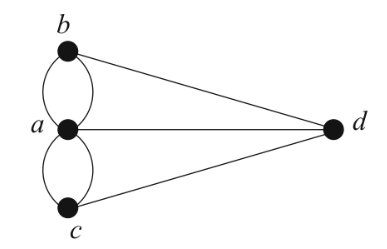
\includegraphics[scale=1]{Illustrations/graph.png}
	\caption{Modell eines ungerichteten Graphen. \citep{graphTheory}}
\end{figure}
\newpage
\subsection{Knoten} % fold
\label{sec:knoten}
Knoten beschreiben Punkte innerhalb eines Graphen, die beispielsweise als Objekte der realen Welt verstanden werden können. Sie können zum Beispiel als geografische Koordinaten dienen, um einen Distanzgraphen zu erstellen, oder als Webseiten, um einen Webgraphen zu erhalten, der die Verbindung verschiedener Webseiten aufzeigt. Innerhalb der Knoten werden verschiedene Typen unterschieden: Zum einen existieren isolierte Knoten ohne Verbindung zu anderen Knoten des Graphen, die zur Identifizierung nicht verbundener Teile eines Netzwerks verwendet werden können. Zum anderen bestehen verbundene Knoten, die mindestens eine Verbindung zu einem anderen benachbarten Knoten aufweisen. Außerdem kann eine indirekte Verbindung entstehen, indem ein Pfad zwischen Ausgangs- und Endknoten existiert, der über mehrere Verbindungen führt.  \citep{graphTheory} \citep{graphapplication}
%subsection knoten (end)

\subsection{Kanten} % fold
\label{sec:kanten}
Kanten dienen in einem Graphen dazu, Knoten miteinander zu verbinden, um eine Relation zwischen ihnen zu visualisieren. Jede Kante besitzt einen Start- und Endknoten, wobei es sich um denselben Knoten handelt kann; in diesem Fall liegt eine Schleife vor. Ebenso wie es verschiedene Arten von Knoten gibt, existieren auch verschiedene Kanten. 
In Abb. 2.1 sind \textit{ungerichtete Kanten}im Graphen zu sehen, Sie die die Knoten auf die trivialste Art verbinden, indem sie ohne Richtung, Gewicht oder andere Beschränkung eine Verbindung herstellen. Durch ungerichtete Kanten entsteht ein ungerichteter Graph. 
\textit{Gerichtete Kanten} werden in Abb. 2.2 (a) durch einen Pfeil visualisiert, der angibt, in welche Richtung der Graph eine Beziehung zwischen den Knoten herstellt. Es ist ebenfalls möglich, dass zwei Knoten eine beidseitige Beziehung durch zwei gerichtete Kanten eingehen, also eine Kante pro Richtung. Ein Graph, der durch gerichtete Kanten verbunden ist, wird ‚gerichteter Graph‘ genannt. Werden Zahlenwerte zu einer Kante hinzugefügt (vgl. Abb 2 (b)), so handelt es sich um eine \textit{gewichteten Kante}. Sie können verwendet werden, um die Strecke zwischen zwei Kanten darzustellen oder die Kosten für die Nutzung der Kante anzugeben. Wird ein Graph mit gewichteten Kanten verbunden, liegt ein gewichteter Graph vor. \citep{graphTheory} \citep{graphapplication}
\begin{figure}[H]
	\centering
	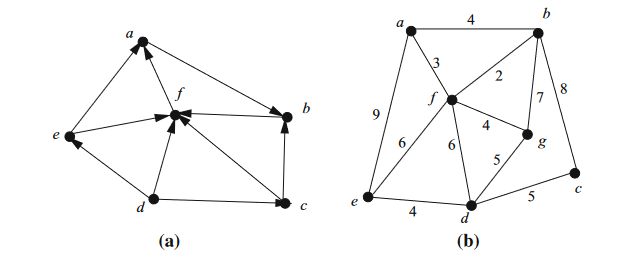
\includegraphics[scale=1]{Illustrations/graph_01.png}
	\caption{Modell eines gerichteten (a) und eines gewichteten Graphen (b). \citep{graphTheory}}
\end{figure}
%subsection kanten (end)

\subsection{Traversierung} % fold
\label{sec:traversierung}
Die Bewegung eines Knoten oder einer Kante zu einem anderen Knoten innerhalb eines Graphen nach vorgegebenen Kriterien wird als Traversierung bezeichnet. Graphdatenbanken bieten in der Regel Traversierungsmechanismen, um Daten miteinander verbundener Knoten effizient abzufragen sowie abzurufen. \cite{graph}
%subsection traversierung (end)


% section graphentheorie (end)

\section{APIs} % (fold)
\label{sec:apigrundlagen}
Nachfolgend werden die Grundlagen von APIs erläutert, wobei die grundlegenden Definitionen sowie die für diese Arbeit relevanten Typen behandelt werden.
\subsection{Definition} % (fold)
\label{sec:grundlegendedefinitionvonapi}
Eine API bezeichnet eine Schnittstelle, die Entwicklern den Zugriff auf Daten und Informationen ermöglicht. Beispiele für häufig genutzte APIs bieten die Twitter- und Facebook-APIs, die für Entwickler zugänglich sind und die Interaktion mit der Software von Twitter sowie Facebook ermöglichen. Zudem erlauben APIs die Kommunikation zwischen Anwendungen und bieten diesen einen Weg, miteinander über ein Netzwerk, überwiegend das Internet, in einer gemeinsamen Sprache zu kommunizieren.  \citep{apistrategyguide}
%subsection grundlegendedefinitionvonapi (end)
\newpage
\subsection{REST API} % (fold)
\label{sec:restapi}
 \textbf{REST} wurde erstmals im Jahr 2000 in einer Dissertation von Roy Fielding beschrieben, wobei es sich um einen Software-Architekturstil für APIs handelt. Dabei basiert REST auf dem ressourcenorientierten Designprinzip, wonach jede Entität als Ressource betrachtet und durch einen eindeutigen Uniform Resource Locator identifiziert wird. Die Architektur fundiert auf sechs grundlegenden Beschränkungen, darunter die Client-Server-Architektur, bei der Client und Server unabhängig voneinander agieren. Einen wesentlichen Bestandteil von REST bildet die Zustandslosigkeit, d. h., jede Anfrage beinhaltet sämtliche für die Verarbeitung erforderlichen Informationen, was die Interaktion zwischen Client und Server vereinfacht. Die Umsetzung der Operationen Create, Read, Update und Delete (CRUD) erfolgt durch die HTTP-Methoden (POST, GET, PUT, DELETE). Das in HTTP integrierte Caching nutzt REST, um die Antwortzeiten und die Leistung zu optimieren, wobei die Möglichkeit besteht, Serverantworten als cachefähig oder nicht cachefähig zu kennzeichnen. Des Weiteren ist eine einheitliche Schnittstelle zu nennen, die die Interaktionen zwischen unterschiedlichen Geräten und Anwendungen erleichtert, worüber hinaus REST ein mehrschichtiges System erfordert, bei dem jede Komponente lediglich mit der unmittelbar vorgelagerten Schicht interagiert. Diesen Prinzipien folgende RESTful-APIs, nutzen HTTP-Anfragen, um Ressourcen effizient zu bearbeiten.  \citep{Fielding2000}  \citep{graphqlreplacerest}

%subsection restapi (end) 
\subsection{GraphQL} % (fold)
\label{sec:graphql}
\textbf{GraphQL} wurde 2012 von Facebook für den internen Gebrauch entwickelt und 2015 als Open-Source-Projekt veröffentlicht. Das Kernkonzept von GraphQL basiert auf clientgetriebenen Abfragen, bei denen der Client die Struktur der Daten präzise definiert und nur die tatsächlich benötigten Daten anfordert. Diese clientseitige Steuerung reduziert die Menge der übertragenen Daten und führt zu effizienteren Netzwerkaufrufen, weil nur die relevanten Informationen übermittelt werden. Im Vergleich zu REST verursacht GraphQL signifikant weniger Overhead, was die Netzwerkperformance optimiert. Die hierarchische Struktur der Abfragen, die die Graphstruktur widerspiegelt, ermöglicht eine intuitive und flexible Datenmodellierung, wobei die starke Typisierung in GraphQL durch ein Schema definiert wird, das die Typen der Daten spezifiziert, was eine verbesserte Validierung der Abfragen und eine klarere Dokumentation erlaubt. Im Gegensatz zu REST, der für verschiedene Operationen mehrere Endpunkte erfordert, nutzt GraphQL nur einen Endpunkt für alle API-Abfragen, was die Komplexität auf der Serverseite reduziert und eine vereinfachte API-Verwaltung ermöglicht. \citep{graphqlreplacerest}
%subsection graphql (end)
% section apigrundlagen (end)

\section{Datenbank} % (fold)
\label{sec:datenbankGrundlagen}
Im Folgenden werden die Grundlagen von Datenbanken behandelt, indem zentrale Definitionen im Zusammenhang mit Datenbanken und die verschiedenen Arten von Datenbanken vorgestellt werden.
\subsection{Definition von Datenbank und Datenbank-Management-System} % (fold)
\label{sec:definitiondatenbank}
Eine Datenbank stellt eine Sammlung von Daten und Informationen dar, die für den einfachen Zugriff gespeichert und organisiert werden, was sowohl die Verwaltung als auch die Aktualisierung der Daten umfasst. Die in der Datenbank gespeicherten Inhalte können nach Bedarf erweitert, gelöscht oder geändert werden. Dabei basiert die Funktionsweise von Datenbanksystemen auf der Abfrage von Informationen oder Daten, woraufhin entsprechende Anwendungen ausgeführt werden. Hier bezeichnet ‚Datenbank-Management-System‘ (DBMS) eine Systemsoftware, die für die Erstellung und Verwaltung von Datenbanken eingesetzt wird. Zu den Funktionalitäten zählen die Erstellung von Berichten, die Kontrolle von Lese- und Schreibvorgängen sowie die Durchführung einer Nutzungsanalyse. Das DBMS fungiert als Schnittstelle zwischen den Endnutzern und der Datenbank, um die Organisation und Manipulation von Daten zu erleichtern, wobei die Kernfunktionen des DBMS die Verwaltung von Daten, des Datenbankschemas, das die logische Struktur der Datenbank definiert, sowie der Datenbank-Engine umfassen, die das Abrufen, Aktualisieren und Sperren von Daten ermöglicht. Diese drei wesentlichen Elemente dienen der Bereitstellung standardisierter Verwaltungsverfahren, der Gleichzeitigkeit, der Wiederherstellung, der Sicherheit und der Datenintegrität.  \citep{9677042}

%subsubsection definitiondatenbank (end)

\subsection{Relationale Datenbank} % (fold)
\label{sec:relationaleDatenbanken}
Relationale Datenbanken basieren auf dem von E. F. Codd entwickelten relationalen Modell und fundieren auf relationaler Algebra sowie dem Tupel-Relational-Kalkül. Sie speichern Daten in einer hochstrukturierten Tabellenform, wobei jede Tabelle aus Zeilen, den sogenannten Tupeln, und Spalten, den sogenannten Attributen, besteht. Jede Zeile repräsentiert einen Datensatz, während jede Spalte durch einen spezifischen Datentyp definiert ist. Diese Struktur ermöglicht eine klare Organisation der Daten und erleichtert deren Verwaltung. Relationale Datenbanken verwenden Primär- und Fremdschlüssel, um Beziehungen zwischen Tabellen herzustellen sowie referenzielle Integrität zu gewährleisten, wodurch die Datenkonsistenz erhalten bleibt. Aufgrund dieser Eigenschaften werden die Tabellen auch als ‚Relationen‘ bezeichnet.

\newpage \noindent
Die bekanntesten relationalen Datenbank Management Systeme (RDBMS) sind Microsoft SQL Server, Oracle MySQL und IBM DB2. Ein RDBMS organisiert alle Daten in tabellarischer Form und bietet Funktionen wie Primärschlüssel zur eindeutigen Identifikation von Datensätzen sowie Indizes, die die Geschwindigkeit der Datenabfragen erhöhen. Darüber hinaus unterstützen RDBMS die Erstellung virtueller Tabellen, die komplexe Abfragen vereinfachen, sowie einen kontrollierten Mehrbenutzerzugriff mit individueller Rechtevergabe. Die Verwendung einer standardisierten SQL ermöglicht die Verwaltung, Abfrage und Manipulation von Daten, wobei die genannten Merkmale die Flexibilität und Benutzerfreundlichkeit relationaler Datenbanken stärken. Ein Vorteil relationaler Datenbanken liegt in ihrer Unterstützung der Prinzipien Atomicity, Consistency, Isolation und Durability (ACID), die Stabilität und Sicherheit bei Transaktionen gewährleisten, was sie für mehrere Anwendungsbereiche geeignet macht. Darüber hinaus bieten sie eine hohe Datenintegrität, reduzieren Redundanz und ermöglichen die einfache Implementierung von Sicherheitsmaßnahmen. Trotz dieser Vorteile stoßen relationale Datenbanken bei bestimmten Anforderungen an ihre Grenzen:. Sie sind selten für hohe Skalierbarkeit geeignet und können mit dem exponentiellen Wachstum von Daten schwer umgehen. Auch die Einrichtung und Wartung solcher Systeme erweist sich häufig als kostspielig und die Verwaltung unstrukturierter Daten wie Multimedia oder Social-Media-Inhalten stellt eine Herausforderung dar. Zudem erschwert die tabellarische Struktur komplexe Datenverknüpfungen und die Integration mehrerer Datenbanken. Aufgrund dieser Einschränkungen führten moderne Anwendungen und Big-Data-Anforderungen zur Entwicklung von NoSQL-Datenbanken, die effektiver auf die Verwaltung unstrukturierter und verteilter Daten ausgelegt sind. Dennoch bleiben relationale Datenbanken aufgrund ihrer Standardisierung, Benutzerfreundlichkeit und ihrer breiten Einsatzmöglichkeiten ein wesentlicher Bestandteil der Datenbanktechnologie.  \citep{relationalDatabase}  \citep{9677042}
%subsection relationaleDatenbanken (end)
\subsection{Graphdatenbanken} % (fold)
\label{sec:graphDatenbanken}
Graphdatenbanken beschreiben spezialisierte Datenbanksysteme, die dem User ein Datenmodell in Form eines Graphen präsentieren. Darüber hinaus enthalten die Graphen Informationen über die Eigenschaften der Knoten und Kanten, was eine flexible und schemafreie Speicherung semistrukturierter Daten ermöglicht. Abfragen in Graphdatenbanken wer- den häufig als Traversal formuliert, wodurch sie gegenüber relationalen Datenbanken erhebliche Geschwindigkeitsvorteile bieten, insbesondere bei komplexen Beziehungsabfragen. Es wird zwischen nativen und nicht nativen Graphdatenbanken unterschieden, wobei native Graphdatenbanken speziell für das Graphmodell entwickelt sind und die Daten intern in Graphenform speichern. Nicht native Graphdatenbanken hingegen verwenden andere Speichertechnologien, beispielsweise relationale Datenbanken, und präsentieren die Daten lediglich in Form von Graphen, um CRUD-Zugriffe zu ermöglichen. Beide Typen gehören zur Kategorie der NoSQL-Datenbanken, die durch den Verzicht auf das starre Tabellenschema relationaler Datenbanken deren Schwächen umgehen. Durch ihre besondere Architektur ermöglichen Graphdatenbanken nicht nur eine effiziente Verarbeitung von Beziehungsdaten, sondern erfüllen auch ACID-Bedingungen und unterstützen Rollbacks, was die Konsistenz der gespeicherten Informationen gewährleistet. Damit stellen sie eine leistungsstarke Alternative zu traditionellen relationalen Datenbanken dar, insbesondere in Anwendungsbereichen mit hochgradig verknüpften Daten. 
\citep{9677042} \citep{graphdb} 
%subsection graphDatenbanken (end)
% section datenbankGrundlagen (end)

% chapter grundlagen (end)
\chapter{Analyse} % (fold)
\label{sec:analyse}

Relationale Datenbanken stoßen in mehreren Bereichen an ihre Grenzen. So können Zugriffszeiten bei großen Datenmengen in relationalen Datenbanken stark ansteigen, während sie in Graphdatenbanken nahezu konstant bleiben, da diese Traversal-basierte Abfragen nutzen. Die Komplexität nimmt mit der Anzahl der Relationen ebenfalls zu, da umfangreiche und schwer überschaubare SQL-Statements erforderlich werden, die oft als "Join Pains" bezeichnet werden. Graphdatenbanken bieten hingegen intuitive und kürzere Abfragesprachen. Darüber hinaus eignen sich relationale Datenbanken trotz ihres Namens oft nur bedingt dazu, Beziehungen zwischen Dateneinträgen effizient abzubilden, da diese häufig über Schlüssel und mehrere Tabellen hinweg konstruiert werden müssen. Graphdatenbanken unterstützen solche Verknüpfungen hingegen nativ.



Ein großer Vorteil relationaler Datenbanken liegt in ihrer Unterstützung der ACID-Prinzipien (Atomicity, Consistency, Isolation, Durability). Diese gewährleisten Stabilität und Sicherheit bei Transaktionen, was sie für viele Anwendungsbereiche geeignet macht. Darüber hinaus bieten sie eine hohe Datenintegrität, reduzieren Redundanz und ermöglichen die einfache Implementierung von Sicherheitsmaßnahmen. Trotz dieser Vorteile stoßen relationale Datenbanken bei bestimmten Anforderungen an ihre Grenzen. Sie sind oft nicht für hohe Skalierbarkeit geeignet und können mit dem exponentiellen Wachstum von Daten schwer umgehen. Die Einrichtung und Wartung solcher Systeme ist häufig kostspielig, und die Verwaltung unstrukturierter Daten wie Multimedia oder Social-Media-Inhalte stellt eine große Herausforderung dar. Zudem erschwert die tabellarische Struktur komplexe Datenverknüpfungen und die Integration mehrerer Datenbanken.

Aufgrund dieser Einschränkungen haben moderne Anwendungen und Big-Data-Anforderungen zur Entwicklung von NoSQL-Datenbanken geführt, die besser auf die Verwaltung unstrukturierter und verteilter Daten ausgelegt sind. Dennoch bleiben relationale Datenbanken aufgrund ihrer Standardisierung, Benutzerfreundlichkeit und breiten Einsatzmöglichkeiten ein wesentlicher Bestandteil der Datenbanktechnologie.

% chapter analyse (end)
\chapter{Datenmodellierung} % (fold)
\label{sec:datamodelling}
Um für das empirische Experiment eine Datenbasis zu schaffen benötigt es ein Datenmodell. Hierbei soll ein möglichst realistisches und flexibles Modell genutzt werden, zudem sollte dieses Verzweigungen aufweisen um verschiedene Abfragekomplexitäten abbilden zu können. In diesem Szenario (vgl. Abb. 3) handelt es sich um ein Projektmanagement-Tool. Es exestieren drei Klassen, welche über drei Beziehungen miteinander verbunden sind. Die Klasse Person modeliert einen Menschen, mit den Attributen Vorname, Nachname und E-Mail. Sie steht mit der Klasse Project in einer n:n-Beziehung, wodurch mehrere Projekte zu einer Person zugeordnet werden können, aber auch mehrere Personen an einem Projekt arbeiten können. In der Klasse Projekt werden nur der Titel und das Datum an welchem das Projekt erstellt wurde gespeichert. Ein Projekt steht in einer 1:n-Beziehung zur Klasse Issue. Dadurch kann einem Issue nur ein Projekt zugeordnet werden, ein Projekt kann aber mehrere Issues beinhalten. Issue speichert Daten wie etwa den Titel, das Erstellngsdatum, den Status und den Grund des Status des Issues. Issue besitzt eine n:n-Beziehung zu Person, wodurch ein Issue von mehreren Personen bearbeitet werden kann und eine Person in mehreren Issues arbeiten kann.
\vspace{1cm}
\label{sec:datenmodell}
\begin{figure}[h!]
	\centering
	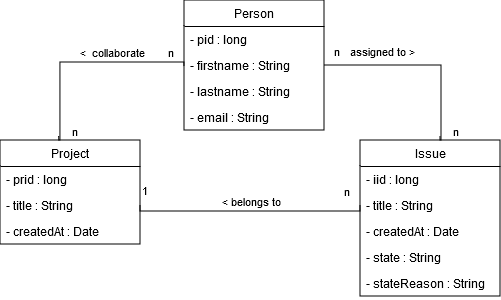
\includegraphics[scale=.8]{Illustrations/class_diagram.png}
	\caption{Klassendiagramm}
\end{figure}


% chapter datamodelling (end)


\chapter{Systemdesign} % (fold)
\label{sec:systemdesign}
Innerhalb dieses Abschnitts sollen die konkreten Technologien beschrieben werden, die gewählt wurden um ein System zu entwickeln welches für Latentztests verwendet werden kann.
\section{Datenbankdesign} % (fold)
Für die Durchführung des Experiments werden zwei Datenbanktypen verwendet, welche nachfolgend mit ihrer konkreten Konfiguration beschrieben werden.
\label{sec:datenbankdesign}
\subsection{Relationales Datenbankdesign} % (fold)
\label{sec:relationalesdatenbankdesign}

\begin{figure}[H]
	\centering
	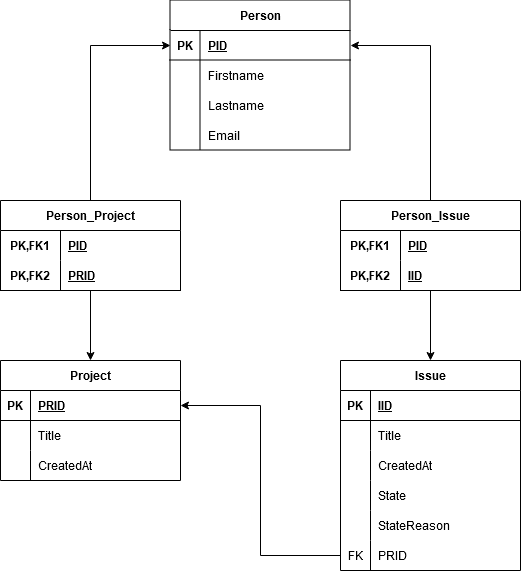
\includegraphics[scale=0.6]{Illustrations/table_diagram.png}
	\caption{Datenbank Diagramm}
\end{figure}
\newpage
\noindent
Um eine relationale Datenbank aus dem gegebenen Datenmodell (Abb. 4.1) zu erstellen muss dieses wie in Abb. 5.1 zu sehen ist angepasst werden, um die Beziehung zwischen \texttt{Person} und \texttt{Project} als auch \texttt{Person} und \texttt{Issue} abzubilden. Somit ergeben sich für die relationale Datenbank fünf Tabellen, welche in einer PostgreSQL Datenbank realisiert werden. PostgreSQL wird verwendet, da es ein leistungsfähiges, objekt-relationales Datenbanksystem bietet welches Open-Source ist und kostenfrei zur Verfügung steht. Die Datenbank wurde mit Beispieldaten befüllt, welche in Abbildung 5.2 bis 5.6 beispielhaft zu sehen sind. Hierbei wurden 500.000 \texttt{Person} als auch \texttt{Project} und \texttt{Issue} Objekte in die Datenbank eingefügt. Durch die Verwendung von Zwischentabellen, wie \texttt{Person\_Issue} und \texttt{Person\_Project}, enthält die relationale Datenbank 2,5 Mio. Tupel, die einen Speicherbedarf von 215MB besitzen. 

\begin{figure}[H]
	\centering
	\begin{tabular}{|l | l | l | l |}
	\hline
	pid & firstname & lastname & email \\
	\hline
	1 & Cecilla & Beningfield & cbeningfield9@wp.com \\
	\hline
	\end{tabular}
	\caption{Tupel der Tabelle Person}
\end{figure}
\begin{figure}[H]
	\centering
	\begin{tabular}{|l | l |}
	\hline
	pid & iid \\
	\hline
	1 & 4894 \\
	\hline
	\end{tabular}
	\caption{Tupel der Tabelle Person\_Issue}
\end{figure}
\begin{figure}[H]
	\centering
	\begin{tabular}{|l | l | l | l | l | l|}
	\hline
	iid & title & createdat & state & statereason & prid \\
	\hline
	1 & Dabfeed & 2023-06-10 00:00:00 & Open & Assigned & 586 \\
	\hline
	\end{tabular}
	\caption{Tupel der Tabelle Issue}
\end{figure}
\begin{figure}[H]
	\centering
	\begin{tabular}{|l | l |}
	\hline
	pid & iid \\
	\hline
	1 & 714 \\
	\hline
	\end{tabular}
	\caption{Tupel der Tabelle Person\_Project}
\end{figure}
\begin{figure}[H]
	\centering
	\begin{tabular}{|l | l | l |}
	\hline
	prid & title & createdat \\
	\hline
	1 & Asoka & 2022-02-17 00:00:00 \\
	\hline
	\end{tabular}
	\caption{Tupel der Tabelle Project}
\end{figure}
\newpage


% subsection relationalesdatenbankdesign (end)
\subsection{Graphdatenbankdesign} % (fold)
\label{sec:graphsdatenbankdesign}
Um eine Graphdatenbank zu erstellen, benötigt man keine definierten Tabellen, da diese die Daten schemafrei speichert. Die Kanten werden bei der Erstellung entsprechend der Objekte benannt, ebenso werden die Beziehungen zwischen den Knoten bei der Erstellung benannt. Als Graphdatenbank wird auf Neo4j zurückgegriffen. Es ist eine der am weitesten verbreiteten Graphdatenbanken und bietet eine hohe Benutzerfreundlichkeit. In Abbildung 5.7 ist eine Demonstration einer Beziehung zwischen jeweils einem Knoten zu sehen. Die Kanten sind als gerichtete Kanten abgebildet, dabei hat \texttt{Person} zwei ausgehende Kanten, \texttt{Project} zwei eingehende und \texttt{Issue} jeweils eine eingehende als auch eine ausgehende Kante. Wie in der relationalen Datenbank wurden auch in der Graphdatenbank 500.000 Knoten pro Objekt erstellt. Hierbei werden jedoch keine Zwischentabellen benötigt, um Beziehungen darzustellen, wodurch in der Datenbank 1,5 Mio. Knoten vorhanden sind, die durch 2,01 Mio. Kanten verbunden sind. Hieraus ergibt sich eine Gesamtgröße von 197MB.


\begin{figure}[H]
	\centering
	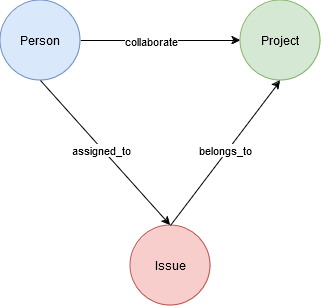
\includegraphics[scale=.8]{Illustrations/graph_diagram}
	\caption{Graph Diagramm}
\end{figure}
% subsection graphdatenbankdesign (end)

% section datenbankdesign (end)
\newpage
\section{Schnittstellendesign} % (fold)
\label{sec:schnittstellendesign}

\subsection{REST}
\label{sec:rest}
Bei REST wird für jedes Testszenario ein separater Endpunkt benötigt. Hierbei wurden sechs verschiedene Endpunkte mit unterschiedlicher Komplexität entworfen.

\begin{itemize}
\item \colorbox{gray!20}{\textbf{HEAD api/resource}} wird verwendet, um einen Head-Request durchzuführen, um die Latenz der API zu bestimmen.
\item \colorbox{gray!20}{\textbf{GET api/issues?counter=x\&?joins=y}}: Hierbei kann die Menge der Ergebnistupel (x) und die Anzahl der Joins(y) die auf der Datenbank durchgeführt werden bei der Anfrage bestimmt werden. Die in Abbildung 5.8 dargestellte Antwort wird hierbei erwartet.
\begin{figure}[H]
\begin{center}
\begin{BVerbatim}
   {
        "iid": 1,
        "title": "Pixope",
        "createdAt": "2024-07-23 00:00:00",
        "state": "Closed"
        "stateReason": "Cancelled"
    },
[...]
\end{BVerbatim}
\end{center}
\caption{GET api/issues?counter=x\&?joins=y Response}
\end{figure}


\item \colorbox{gray!20}{\textbf{GET api/persons/:pid}}: Dieser Endpunkt ermöglicht das Abrufen einer bestimmten \texttt{Person} anhand ihrer \texttt{ID}. Die API liefert dabei ein JSON-Objekt zurück, dass die \texttt{Person} mit den Attributen \texttt{Firstname, Lastname} und \texttt{E-Mail} beschreibt. (Abb. 5.9)
\begin{figure}[H]
\begin{center}
\begin{BVerbatim}
{
    "pid": 10,
    "firstname": "Cecilla",
    "lastname": "Beningfield",
    "email": "cbeningfield9@wp.com"
}
\end{BVerbatim}
\end{center}
\caption{GET api/persons/:pid Response}
\end{figure}

\item Mit dem Endpunkt  \colorbox{gray!20}{\textbf{GET api/persons}} können alle in der Datenbank gespeicherten \texttt{Person} Objekte abgerufen werden. Die Antwort umfasst 5000 \texttt{Project} Objekte im JSON-Format. (Abb. 5.10)

\begin{figure}[H]
\begin{center}
\begin{BVerbatim}
[
    {
        "pid": 1,
        "firstname": "Ruby",
        "lastname": "Burchatt",
        "email": "rburchatt0@msn.com"
    },
	[...]
    {
        "pid": 5000,
        "firstname": "Murdoch",
        "lastname": "Simonitto",
        "email": "msimonittorr@google.ca"
    }
]
\end{BVerbatim}
\end{center}
\caption{GET api/persons Response}
\end{figure}

\item Der Endpunkt \colorbox{gray!20}{\textbf{GET api/persons/:pid/projects/issue}} erhöht die Komplexität, da hier nicht nur auf ein einzelnes Objekt zugegriffen wird. Stattdessen erfordert die Abfrage mehrere Objekte, die miteinander in Abhängigkeit stehen, um die Anfrage zu bearbeiten. Die Antwort umfasst alle  \texttt{Issue} Objekte, die in  \texttt{Project} Objekten vorhanden sind in der eine  \texttt{Person} mitwirkt. (Abb. 5.11)
\begin{figure}[H]
\begin{center}
\begin{BVerbatim}
[
   {
        "iid": 1,
        "title": "Pixope",
        "createdAt": "2024-07-23 00:00:00",
        "state": "Closed"
        "stateReason": "Cancelled"
    },
    {
        "iid": 2876,
        "title": "Zoomlounge",
        "createdAt": "2020-08-26 00:00:00",
        "state": "Open"
        "stateReason": "Bug"
    },
]
\end{BVerbatim}
\end{center}
\caption{GET api/persons/:pid/projects/issue Response}
\end{figure}

\item \colorbox{gray!20}{\textbf{POST api/persons/:pid/projects/:prid/issues}}: Dieser Endpunkt ermöglicht das Erstellen eines neuen  \texttt{Issue} in der Datenbank, um nicht nur Abfragen zu testen, sondern auch das Hinzufügen von Daten. Im Body der Anfrage wird ein  \texttt{Issue} Objekt im JSON-Format übergeben. (Abb. 5.12) 
\newline
\begin{figure}[H]
\begin{center}
\begin{BVerbatim}
{
    "title":"test",
    "createdAt":"2023-02-21T00:00:00",
    "state":"Open",
    "stateReason":"Bug"
}
\end{BVerbatim}
\end{center}
\caption{POST api/persons/:pid/projects/:prid/issues Body}
\end{figure}
Die Antwort enthält das erstellte \texttt{Issue}, das eine gültige  \texttt{ID}, sowie Verknüpfungen zu dem zugehörigen  \texttt{Project} und der  \texttt{Person} beinhaltet. (Abb. 5.13)
\begin{figure}[H]
\begin{center}
\begin{BVerbatim}
{
    "iid": 5207,
    "title": "test",
    "createdAt": "2023-02-21T00:00:00",
    "state": "Open",
    "stateReason": "Bug",
    "project": {
        "prid": 12,
        "title": "Y-find",
        "createdAt": "2021-01-10T00:00:00"
    },
    "assignee"{
        "pid": 1,
        "firstname": "Ruby",
        "lastname": "Burchatt",
        "email": "rburchatt0@msn.com"
    },
}
\end{BVerbatim}
\end{center}
\caption{POST api/persons/:pid/projects/:prid/issues Response}
\end{figure}
\end{itemize}

% section rest (end)

\subsection{GraphQL}
GraphQL unterscheidet sich bei der Art der Anfragen sehr stark zu REST. Es wird nur über den Endpunkt \colorbox{gray!20}{POST api/graphql} angesprochen. Hierüber werden sowohl Querys als auch Mutations abgedeckt. Die Anfragen werden im Body mithilfe der GraphQL Query Language definiert, welche JSON sehr ähnlich ist. Die in 5.2.1 definierten REST-Endpunkte wurden in GraphQL nachgebildet, sodass sie dieselbe Antwort liefern. Für einen HEAD Request bietet GraphQL nativ jedoch keine Lösung, weshalb in GraphQL APIs der HEAD Request identisch wie in den REST APIs implementiert wurde.
Der parametrisierte Endpunkt aus der REST-API wurde in GraphQL wie in Abb. 5.14 dargestellt umgesetzt. Hierbei sind bei  \texttt{Counter} Werte zwischen 0 und 1,5 Mio und bei  \texttt{Joins} Werte zwischen 0 und 3 möglich.

\begin{figure}[H]
\begin{center}
\begin{BVerbatim}
query{
    issuesCount(counter: 10, joins: 1){
	iid
	title 
	createdAt 
	state 
	stateReason
    }
}
\end{BVerbatim}
\end{center}
\caption{GraphQL Query GET api/issues?counter=x\&?joins=y}
\end{figure}
\noindent
Die in Abbildung 5.15 dargestellte Query ist dem REST-Endpunkt \colorbox{gray!20}{GET api/persons/:pid} äquivalent. Hierbei wird ebenfalls eine \texttt{ID} übergeben, allerdings können die Felder, die in der Antwort enthalten sind, explizit gewählt werden. In diesem Beispiel wurden die  \texttt{PID},  \texttt{Firstname},  \texttt{Lastname} als auch die  \texttt{E-Mail} gewählt, um dieselbe Antwort wie der REST-Endpunkt zu erhalten. 
\begin{figure}[H]
\begin{center}
\begin{BVerbatim}
query{
    person(id : 10){
	pid
	firstname
	lastname
	email
    }
}
\end{BVerbatim}
\end{center}
\caption{GraphQL Query equivalent zu GET api/persons/:pid}
\end{figure}
\noindent
Der REST-Endpunkt \colorbox{gray!20}{GET api/persons} wird von der GraphQL Query in Abbildung 5.16 repräsentiert. Hierbei werden dieselben Felder selektiert wie in der vorherigen Abfrage, jedoch wird hierbei die Query \colorbox{gray!20}{persons} angesprochen, wodurch alle  \texttt{Person} Objekte der Datenbank abgerufen werden.
\begin{figure}[H]
\begin{center}
\begin{BVerbatim}
query {
    persons {
        pid
        firstname
        lastname
        email
    }
}
\end{BVerbatim}
\end{center}
\caption{GraphQL Query equivalent zu GET api/persons}
\end{figure}
\noindent
Abbildung 5.17 zeigt die GraphQL Query, welche dem REST-Endpunkt \colorbox{gray!20}{GET api/persons/} \colorbox{gray!20}{:pid/projects/issue} entspricht. Hierbei werden die im Schema definierten Querys geschachtelt, um eine Abfrage zu erhalten, welche die Abhängigkeiten zwischen den Objekten repräsentiert.
\begin{figure}[H]
\begin{center}
\begin{BVerbatim}
query{
    person(id : 10){
        projects{
	    issues{
		iid
		title
		createdAt
		state
		stateReason
	    }
        }
    }
}
\end{BVerbatim}
\end{center}
\caption{GraphQL Query equivalent zu GET api/persons/:pid/projects/issue}
\end{figure}
\noindent
Um den REST-Endpunkt \colorbox{gray!20}{POST api/persons/:pid/projects/:prid/issues} nachzubilden wurde die in Abb. 5.18 dargestellte Mutation entwickelt. Hierbei wird ein Input Objekt definiert, welches die Attribute beinhaltet, die zur Erstellung des Issues benötigt werden. Danach kann, wie auch in den zuvor beschriebenen Querys, selektiert werden, welche Felder in der Antwort enthalten sind.
\begin{figure}[H]
\begin{center}
\begin{BVerbatim}
mutation{
    createIssue(input:{
	title : „Bug in Login“
	createdAt : „2024-12-03T12:30:00
	state : „Open“
	stateReason : „Error in Login“
	prid: 80
	pid: 10
	}){
	iid
	title
	state
	stateReason
	createdAt
    }
}
\end{BVerbatim}
\end{center}
\caption{GraphQL Query equivalent zu POST api/persons/:pid/projects/:prid/issues}
\end{figure}

\label{sec:graphql}
% section graphql (end)

% section schnittstellendesign (end)
\section{Testumgebung} % (fold)
\label{sec:testumgebung}
Zur Ermittlung der Latenzzeiten werden API-Abfragen durchgeführt, bei denen die Antwortzeiten in Millisekunden protokolliert werden. Dafür wird eine Testumgebung mit zwei unterschiedlichen Endgeräten benötigt, um die Last auf mehrere Geräte zu verteilen. Die APIs laufen auf einem Server in Frankfurt, der mit 4 Kernen, 24 GB Arbeitsspeicher, einer 1 Gbit-Internetverbindung und Ubuntu 22.04 als Betriebssystem ausgestattet ist.
\newline
Die Abfragen erfolgen von einem PC mit 8 Kernen, 32 GB Arbeitsspeicher, einer 50 Mbit-Internetverbindung und Windows 10 als Betriebssystem. Die durchschnittliche Latenz (Ping) zwischen Server und PC beträgt 24 ms. Da ein Ping jedoch nur auf ISO-Schicht 3 agiert, wird vor jedem Testdurchlauf mithilfe von HEAD-Requests, die in 5.2.1 beschrieben wurden, eine Latenz zwischen den Endgeräten ermittelt, die alle ISO-Schichten durchläuft. Um Schwankungen in der Netzwerkauslastung und der Systembelastung zu minimieren, werden pro Testszenario und API jeweils 100 Anfragen ausgeführt. Insgesamt ergibt dies bei 4 APIs und 25 Testszenarien eine Datengrundlage von 10.000 Latenzzeiten.


% section testumgebung (end)


% chapter Systemdesign (end)
\chapter{Implementierung} % (fold)
\label{sec:implementierung}
Nachfolgend soll die Implementierung der verschiedenen APIs, sowie die Grundprinzipien während der Implementierung, beschrieben werden. Der Source Code der Implementierung ist unter MIT Lizenz auf Github veröffentlicht. \citep{me}
\section{Grundprinzipien während der Implementierung} % (fold)
\label{sec:prinzipien}
Im Rahmen der Implementierung dieser Anwendung wurden verschiedene Grundprinzipien beachtet, die sowohl die Qualität als auch die Erweiterbarkeit der Anwendungen  sicherstellen. Die Wahl der verwendeten Technologien sowie die Anwendung bewährter Praktiken standen dabei im Vordergrund. Als Basis für die Entwicklung wurde Java JDK 17.0.10 Corretto gewählt, da diese Version eine Long-Term-Support (LTS)-Version darstellt und damit eine stabile und sichere Grundlage für die Entwicklung bietet. Amazon Corretto bietet eine optimierte JVM, wodurch alle Softwarebestandteile auf jeder Plattform mit einer zertifizierten JAVA Virtual Machine lauffähig sind. Ergänzt wurde das JDK durch Spring Boot Version 3.3.4, eine weit verbreitete Plattform für die Entwicklung von Webanwendungen und Microservices. Spring Boot ermöglicht eine schnelle und einfache Konfiguration von Anwendungen und vereinfacht den Entwicklungsprozess durch das Automatisieren von häufig auftretenden Aufgaben, wie etwa der Konfiguration von Servern und Datenbankverbindungen.
\noindent
Ein zentrales Konzept während der Implementierung war die Verwendung von Dependency Injection. Diese Technik sorgt dafür, dass die Abhängigkeiten zwischen den einzelnen Komponenten der Anwendung nicht hart kodiert sind, sondern zur Laufzeit durch den DI-Container von Spring injiziert werden. DI fördert die Entkopplung von Komponenten, was zu einer besseren Testbarkeit, Flexibilität und Wartbarkeit des Codes führt. Da der Code durch DI in unabhängige, gut getestete Module unterteilt wird, lässt er sich leicht erweitern und an geänderte Anforderungen anpassen. Zudem trägt DI zur Verbesserung der Lesbarkeit des Codes bei, da Abhängigkeiten nicht explizit im Konstruktor oder an anderen Stellen erstellt werden müssen.
\noindent
Die Implementierung der Anwendung erfolgte unter der Berücksichtigung von Best Practices, die die Qualität des Codes sicherstellen und eine effiziente, langfristige Wartung ermöglichen. Ein wesentlicher Aspekt war hierbei die Modularität der Lösung. Die Anwendung wurde so strukturiert, dass jede Komponente eine klare, abgegrenzte Verantwortung übernimmt. Dies sorgt nicht nur für eine bessere Nachvollziehbarkeit des Codes, sondern erleichtert auch das Testen und die Erweiterung von Funktionalitäten. Bestehende Komponenten können so problemlos durch neue ersetzt oder erweitert werden, ohne die gesamte Anwendung zu beeinträchtigen.




% section prinzipien (end)

\section{Post REST} % (fold)
\label{sec:postrest}
In dieser Arbeit steht "PostREST" für die PostgreSQL REST-API, die eine Schnittstelle für den Zugriff auf eine PostgreSQL-Datenbank über HTTP-Anfragen bietet. Diese API implementiert eine Reihe von Endpunkten, die in Abschnitt 5.2.1 der Arbeit definiert sind. Diese Endpunkte sind dafür verantwortlich, bestimmte Anfragen zu bearbeiten und entsprechende Antworten zurückzugeben.
\noindent
Die zentrale Komponente, die dafür sorgt, dass die Endpunkte korrekt verarbeitet werden, ist die Controller-Klasse(vgl Abb. 6.1). In dieser Klasse sind die Endpunkte integriert, wobei jeder Endpunkt mit seinen spezifischen Pfadvariablen und den Rückgabewerten versehen ist. Die Controller-Klasse übernimmt die Aufgabe, die richtigen Methoden auszuführen, wenn eine Anfrage an einen bestimmten Endpunkt gestellt wird.
\noindent
Der PostrestController ist die konkrete Implementierung des Controllers, der die Geschäftslogik verarbeitet. Er ruft den DBService auf, welcher das Interface IDBService implementiert. Das Interface definiert die Methoden, die notwendig sind, um Daten aus den zugrunde liegenden Datenbanken abzurufen. Diese Methoden kapseln die Logik für den Datenbankzugriff und sind so gestaltet, dass sie von der Controller-Klasse verwendet werden können, um die richtigen Informationen zu erhalten.
\noindent
Die Kommunikation zwischen den verschiedenen Schichten der Anwendung erfolgt durch Dependency Injection. Das bedeutet, dass die verschiedenen Komponenten nicht direkt in der Controller-Klasse erzeugt werden, sondern von außen in die Klasse injiziert werden. In diesem Fall werden die Repositorys der verschiedenen Entitäten in die Controller-Klasse injiziert. Diese Repositorys sind verantwortlich für den direkten Datenbankzugriff und beinhalten die notwendigen Methoden und SQL-Abfragen, die zum Abrufen und Verwalten der Daten in der Datenbank erforderlich sind.
\noindent
Nachdem die Daten erfolgreich aus der Datenbank abgefragt wurden, werden sie durch die Hierarchie der Anwendung weitergegeben. Der PostrestController sorgt dafür, dass die abgerufenen Daten in das gewünschte Format für die API-Antwort umgewandelt werden. Dies ist in diesem Fall das JSON-Format, dass dann dem Nutzer der API als Antwort übermittelt wird. Diese Antwort enthält die angeforderten Informationen, die der Nutzer über die API abgefragt hat.
\begin{figure}[H]
	\centering
	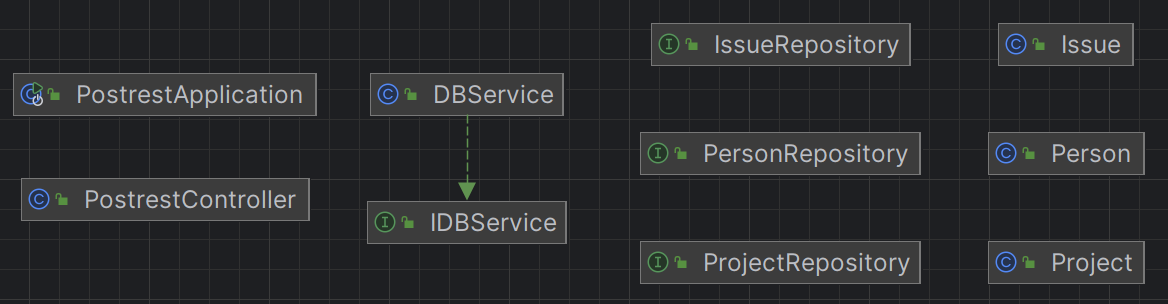
\includegraphics[scale=0.5]{Illustrations/postrest.png}
	\caption{Java Klassen PostREST}
\end{figure}
% section postrest (end)

\section{Post Graph} % (fold)
\label{sec:postgraph}
Hierbei handelt es sich um eine GraphQL-API, die mit einer PostgreSQL-Datenbank verbunden ist. Das Schema, das die Arbeitsweise der API beschreibt, wird – wie bei GraphQL üblich – in der Datei schema.graphqls definiert. In dieser Datei sind die verschiedenen Datentypen sowie die möglichen Queries und Mutationen beschrieben, die zur Abfrage und Bearbeitung der Daten verwendet werden können. 
\noindent
In den folgenden Abbildungen sind Beispiele für einen Typ, verschiedene Queries und eine Mutation dargestellt, wie sie in der schema.graphqls-Datei definiert sind:
\begin{figure}[H]
\begin{center}
\begin{BVerbatim}
type Issue{
    iid : ID!
    title : String
    createdAt : String
    state : String
    stateReason : String
}
\end{BVerbatim}
\end{center}
\caption{Type aus der Schema.graphqls}
\end{figure}
\begin{figure}[H]
\begin{center}
\begin{BVerbatim}
type Query{
    persons: [Person]
    person(id:ID!): Person
    projects: [Project]
    project(id:ID!) : Project
    issues : [Issue]
    issue(id: String): Issue
}
\end{BVerbatim}
\end{center}
\caption{Queries aus der Schema.graphqls}
\end{figure}
\begin{figure}[H]
\begin{center}
\begin{BVerbatim}

type Mutation {
    createIssue(input: IssueInput): Issue
}
\end{BVerbatim}
\end{center}
\caption{Mutation aus der Schema.graphqls}
\end{figure}
\newpage
\noindent
Die zentrale Komponente für die Verarbeitung von Anfragen ist die Java-Klasse Query(vgl. Abb. 6.5). In dieser Klasse werden Methoden implementiert, die die Bearbeitung der Anfragen gemäß den Strukturen in der schema.graphqls-Datei ermöglichen. Diese Methoden greifen auf die Repositories der Modelklassen zu, um Datenbankoperationen durchzuführen. Die Repositories enthalten die erforderlichen Methoden und Logiken, um Daten in der PostgreSQL-Datenbank zu lesen oder zu ändern.
\noindent
Ein hervorstechendes Merkmal von GraphQL ist der Einsatz von Resolvern. Diese kommen zum Einsatz, um Felder zu verarbeiten, die auf Daten aus anderen Quellen oder Datenbanken basieren. Resolver stellen sicher, dass die relevanten Daten korrekt abgerufen und in der gewünschten Struktur zurückgegeben werden.
\noindent
Die Repositories werden in die benötigten Klassen injiziert, sodass sie nicht direkt innerhalb der Anwendung erstellt werden müssen.
\noindent
Nach erfolgreicher Bearbeitung einer Anfrage liefert die GraphQL-API die Daten im vorgegebenen GraphQL-Format an den Nutzer zurück. Dies gewährleistet eine flexible und leistungsfähige Schnittstelle zur Abfrage und Manipulation der Daten in der zugrunde liegenden PostgreSQL-Datenbank.
\begin{figure}[H]
	\centering
	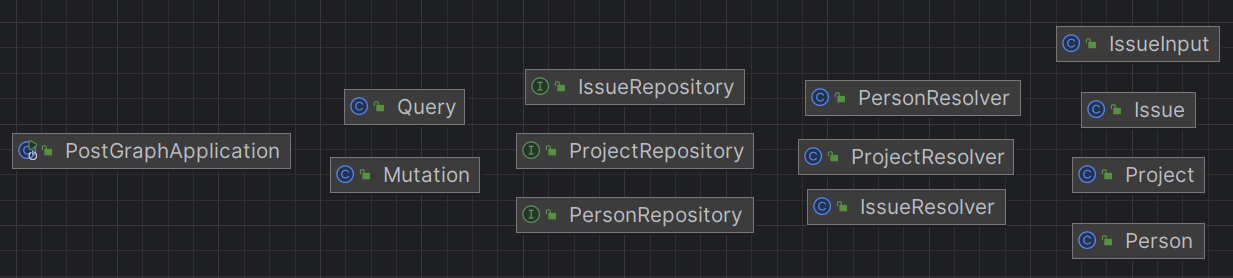
\includegraphics[scale=0.5]{Illustrations/postgraph.png}
	\caption{Java Klassen PostGraph}
\end{figure}
% section postgraph (end)

\section{Neo4REST} % (fold)
\label{sec:neo4rest}
Neo4REST ist eine REST-API, die den Zugriff auf eine Neo4j-Datenbank ermöglicht. Analog zur Struktur von PostREST bietet Neo4REST eine Reihe von Endpunkten, die zur Bearbeitung spezifischer Anfragen und zur Rückgabe der entsprechenden Antworten dienen. Die Details dieser Endpunkte sind in Abschnitt 5.2.2 definiert.
\noindent 
Die Verarbeitung der Endpunkte wird durch die zentrale Controller-Klasse sichergestellt (vgl. Abb. 6.7). Wie bei PostREST sind hier die spezifischen Pfadvariablen, Parameter und Rückgabewerte der Endpunkte definiert. Die Controller-Klasse sorgt dafür, dass die passenden Methoden aufgerufen werden, sobald eine Anfrage an einen der Endpunkte gestellt wird.
\noindent 
Der Neo4RestController übernimmt dabei die Geschäftslogik und delegiert datenbankbezogene Aufgaben an den DBService, der das Interface IDBService implementiert. Dieses Interface definiert die für den Zugriff auf die Neo4j-Datenbank erforderlichen Methoden. Die Umsetzung der konkreten Abfragen erfolgt über Repositorys, die für die Durchführung der Cypher-Abfragen zuständig sind. Diese Repositorys abstrahieren den Datenbankzugriff und bieten wiederverwendbare Methoden, um auf die in Neo4j gespeicherten Daten zuzugreifen oder sie zu ändern.
\noindent 
Die in der Datenbank abgefragten Informationen werden, wie auch bei PostREST, durch die Schichten der Anwendung weitergeleitet und im Controller in das JSON-Format umgewandelt, bevor sie als API-Antwort zurückgegeben werden. So stellt Neo4REST sicher, dass der Nutzer die angeforderten Informationen oder den Status einer Operation im passenden Format erhält.
\begin{figure}[H]
	\centering
	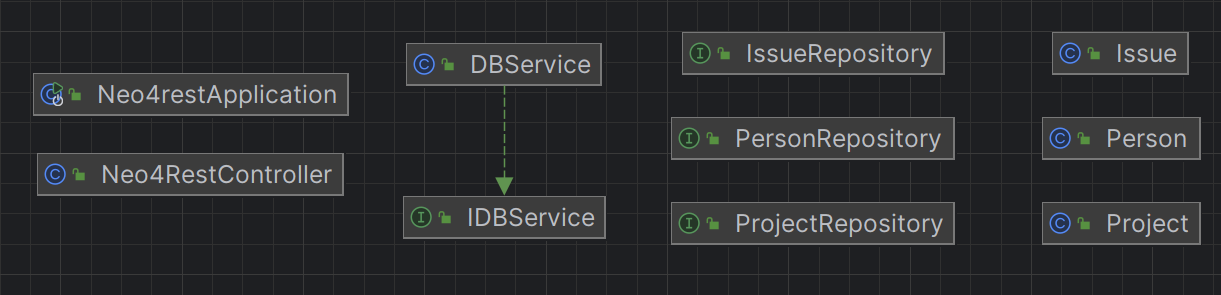
\includegraphics[scale=0.5]{Illustrations/neo4rest.png}
	\caption{Java Klassen Neo4REST}
\end{figure}
% section neo4rest (end)

\section{Neo4Graph} % (fold)
\label{sec:neo4graph}
Die Neo4Graph-API ist eine GraphQL-API, die mit einer Neo4j-Datenbank verbunden ist. Das Schema, das bereits in der PostGraph-API beschrieben wurde, wird auch in Neo4Graph auf ähnliche Weise implementiert. Wie bei PostGraph kommen auch hier Cypher-Abfragen zum Einsatz, um mit der Neo4j-Datenbank zu interagieren. Die Methoden nutzen die Neo4j-Clientbibliothek, um Knoten und Kanten effizient zu durchsuchen und Datenbankoperationen durchzuführen.
\noindent
Ein weiteres gemeinsames Merkmal beider APIs ist der Einsatz von Resolvern. In Neo4Graph werden diese ebenfalls verwendet, um Felder zu bearbeiten, die auf Beziehungen oder aggregierten Daten im Graphen basieren. Resolver sorgen dafür, dass die benötigten Daten korrekt abgerufen und in der gewünschten Struktur zurückgegeben werden.
\noindent
Nach der Bearbeitung einer Anfrage liefert die GraphQL-API die Daten im standardisierten GraphQL-Format an den Nutzer, was eine konsistente und leistungsfähige Schnittstelle zur Abfrage und Bearbeitung der Daten in der Neo4j-Datenbank sicherstellt

\begin{figure}[H]
	\centering
	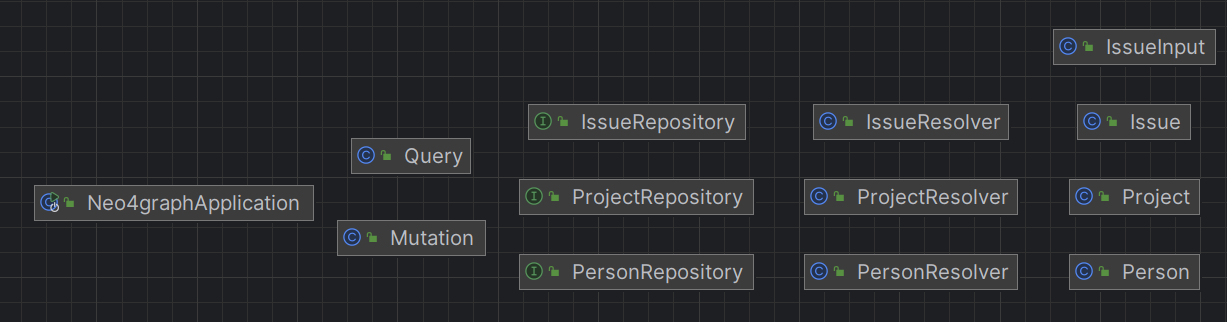
\includegraphics[scale=0.5]{Illustrations/neo4graph.png}
	\caption{Java Klassen Neo4Graph}
\end{figure}
% section neo4graph (end)
\section{API-Response Test} % (fold)
\label{sec:test}
Eine Anwendung wurde entwickelt, um API-Anfragen von einem entfernten System durchzuführen. Diese Anwendung enthält für jeden Endpunkt eine Methode(vgl. Abb. 6.8), die jeweils 100 Abfragen in einer Schleife ausführt. Falls für eine Abfrage eine ID erforderlich ist, wird diese mithilfe der Klasse Random aus java.util.Random generiert. Die Abfragen für den parametrisierten Endpunkt werden mit den Joins von 0 bis 3 und den Ergebnistupeln 1, 100, 1000, 10.000 und 100.000 durchgeführt. Die Abfragezeit wird ermittelt, indem die aktuelle Systemzeit in Millisekunden unmittelbar vor der Ausführung der Abfrage erfasst und von der Zeit nach Abschluss der Abfrage abgezogen wird.
\begin{figure}[H]
	\centering
	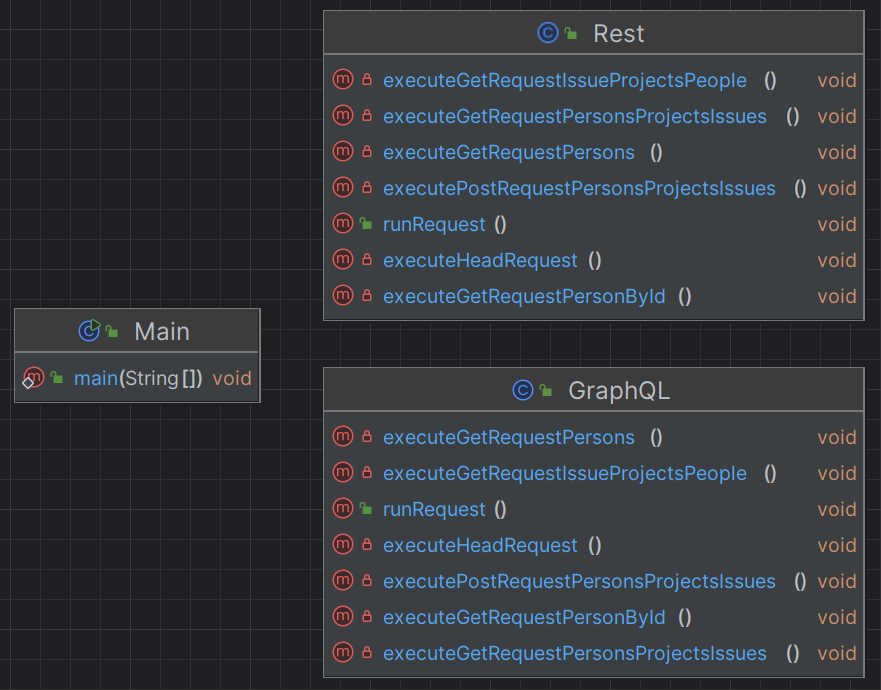
\includegraphics[scale=0.5]{Illustrations/apiresponsetest.png}
	\caption{Java Klassen Neo4Graph}
\end{figure}
% section test (end)
% chapter implementierung (end)
\chapter{Ergebnisse} % (fold)
\label{sec:ergebnisse}
Im Nachfolgenden werden die Ergebnisse der Latenztests der oben eingeführten APIs dargestellt. Die konkreten Zahlen auf denen die Grafiken beruhen sind im Kapitel Appendix zu finden.

\noindent
Zunächst wurde, wie in Abbildung 7.1 zusehen, mittels HEAD Request ermittelt, ob die API verfügbar ist und welche Latenz zwischen Client und Server entsteht, ohne eine Datenabfrage auszuführen. Hierbei kann man beobachten, dass Die Latenz von PostGraph und Neo4Graph sehr dich beieinander liegen. REST basierende APIs hatten in diesem Experiment eine Latenz die deutlich mehr Variation in der Latenz lieferte.

\noindent
Daraufhin wurden die Latenzen des parametrisierten API-Endpunktes ermittelt. In den Abbildungen 7.2 bis 7.5 wurden diese Ergebnisse in einem Koordinatensystem dargestellt. Die x-Achse repräsentiert die Menge der Tupel, welche angefordert wurden. Aufgrund der hohen Menge der Ergebnistupel wurde diese Achse logarithmisch Dargestellt. Auf der z-Achse ist die Latenz in Millisekunden zu sehen. Die verschiedenen Graphen innerhalb der Abbildungen beschreiben die Menge der Joins, bei relationalen Datenbanken, oder Edges, bei Graphdatenbanken. Rot (Kreis) steht hierbei für null, Blau(Quadrat) steht für eins und Orange (Diamant) steht hierbei für zwei. 
\newline
Bei PostREST (vgl. Abb. 7.2) steigt somit die Latenz mit der Menge der Ergebnistupeln exponentiell an. Zudem ist zu erkennen, dass bei einer Menge von 100.000 Ergebnistupeln die Menge der Joins deutlich Einfluss auf die Latenz nehmen. Hierbei ist eine Anfrage die weniger Joins verwendet (Rot) mit 426,5 Millisekunden deutlich performanter, als eine Abfrage die mehrere Joins (Orange) verwendet, welche 492,5 Millisekunden benötigt. Bei niedrigerer Tupelzahl wirken sich Joins nicht, bzw. nur in sehr geringen Maß auf die Latenz der Anfrage aus.
\newline
PostGraph zeigt in Abbildung 7.3 ein ähnliches Bild, jedoch mit einer deutlich höheren Latenz bei einer Anfragengröße von 100.000 Tupel. Die GraphQL API ist hier mit 1831 Millisekunden um einen Faktor von 3,7 langsamer als die REST API, welche auf der selben Datenbank basiert.
\newline
Bei Verwendung einer Neo4j Datenbank in Kombination mit einer REST-API (vgl. Abb. 7.4) fällt auf, dass die Anfragen mit geringer und hoher Komplexität, sowie geringer Tupelzahl eine sehr ähnliche Latenz aufweisen. Bei höherer Tupelzahl liegt die Anfragedauer jedoch deutlich höher, als mit einer relationalen Datenbank. Hierbei erkennt man jedoch, dass Anfragen welche mehrere Edges nutzen schneller bearbeitet werden können. So benötigt eine Anfrage, welche ohne das Nutzen einer Kante auskommt 1673 Millisekunden. Wenn man nun die Komplexität erhöht und für die Anfrage  zwei Edges verwendet benötigt diese lediglich 1371 Millisekunden.
 \newline
Behält man nun die Datenbasis bei und nutzt eine GraphQL API (vgl. Abb. 7.5) fällt auf, dass erneut die Anfragedauer bei hoher Tupelzahl deutlich über der einer REST-API liegt. Ebenfalls ist hier zu beobachten, dass komplexere Anfragen schneller bearbeitet werden, als weniger komplexe.
\newline
\noindent
Wie in Abbildung 7.6 zusehen ist, hat die PostgreSQL REST-API eine höhere Latenzzeit als die GraphQL PostgeSQL. Dies deutet darauf hin, dass die GraphQL API bei der Abfrage eines spezifischen Personenobjekts, anhand der Personen-ID in Kombination mit einer relationalen Datenbank effizientere Abfragen und eine bessere Performance bei der Verarbeitung bietet. Ähnliches zeigt sich bei einer Neo4j Datenbank. Auch hier hat die Neo4j GraphQL API niedrigere Latenzzeiten als die REST-API. Allerdings sind die Latenzen bei Neo4j minimal höher als bei dem relationalen Pendant. Das deutet darauf hin, dass Postgres bei dieser Anfrage eine performantere Verarbeitung von Abfragen ermöglicht. Zusammenfassend kann man für diese Anfrage sagen, dass GraphQL sowohl in Kombination mit einer relationalen, als auch einer Graphdatenbank eine niedrigere Latenz aufweist. Zudem ist Postgres bei dieser Anfrage insgesamt ein wenig performanter als Neo4j.
\newline
In Abbildung 7.7 sind die Latenzen für die komplexere Anfrage, die 5000 Personenobjekte aus der Datenbank zurückliefert dargestellt. GraphQL hat hierbei sowohl bei der relationalen Datenbank als auch bei der Graphdatenbank im Median eine niedrigere Latenz. REST ist somit in beiden Fällen die weniger performantere API.
\newline
Wenn nun die Anfragekomplexität steigt, wodurch sich die Abhängigkeit zwischen den Objekten in der Datenbank erhöht, ist deutlich zu sehen, dass die Streuung bei der Postgres GraphQL API höher ist als bei allen anderen APIs (vgl Abb.7.8). Der Median liegt jedoch deutlich niedriger. Die Neo4j REST-API liegt in diesem Fall deutlich über allen anderen APIs. Gefolgt von der PortgeSQL REST-API.Beide GraphQL APIs weißen erneut eine deutlich niedrigere Latenz auf.
\newline
Bei der Speicherung in eine Datenbank ist ein deutlich anderes Bild zu sehen. Wie in Abbildung 7.9 zusehen, ist hierbei die Postgres REST-API diejenige mit der geringsten Latenz. Dicht gefolgt von der Postgres GraphQL API. Eine deutlich höhere Latenz ist bei den Neo4j APIs zu erkennen. Hierbei ist allerdings die GraphQL API die performantere.


\begin{figure}[htbp]
 \centering
	\begin{tikzpicture}
	    \begin{axis}[
	        boxplot/draw direction=y, 
	        xlabel={API}, 
	        ylabel={ms}, 
	        xtick={1,2,3,4}, 
	        xticklabels={Post Rest, Post Graph, Neo4 Rest, Neo4 Graph}, 
	        ymin=50, ymax=65,
	       ytick distance=1,
                  width=15cm,
	       height= 18cm
	    ]
	       \addplot+[
	            boxplot prepared={
	                median=52,
	                upper quartile=55,
	                lower quartile=52, 
	                upper whisker=59,
	                lower whisker=51
	            },
	            draw=black
	        ] coordinates {};
	        \addplot+[
	            boxplot prepared={
	                median=53,
	                upper quartile=53,
	                lower quartile=53, 
	                upper whisker=54,
	                lower whisker=52
	            },
	            draw=black
	        ] coordinates {};
	         \addplot+[
	            boxplot prepared={
	                median=52,
	                upper quartile=58,
	                lower quartile=52, 
	                upper whisker=63,
	                lower whisker=51
	            },
	            draw=black
	        ] coordinates {};
	       \addplot+[
	            boxplot prepared={
	                median=52,
	                upper quartile=53,
	                lower quartile=52, 
	                upper whisker=54,
	                lower whisker=51
	            },
	            draw=black
	        ] coordinates {};
	    \end{axis}
	\end{tikzpicture}
\caption{HEAD /api/resource}
\end{figure}




\begin{figure}
\centering
\begin{tikzpicture}[scale=1.9]
\begin{axis}[
    axis lines = middle,
    xlabel = {x},
    ylabel = {y},
    zlabel = {z},
    xmode = log,
    width=10cm,
    height=10cm,
    grid = major,
    enlarge x limits = true,
    view={0}{0},
    ymin=0, ymax=3,  
]
% Linie und Punkte für die ersten Punkte (rot)
\addplot3+[
    only marks, 
    mark=*,
    red,
    mark options={fill=red} % Innere des Punktes rot färben
] coordinates {
    (1, 0, 111)
    (100, 0, 121)
    (1000, 0, 135)
    (10000, 0, 272)
    (100000, 0, 426.5)
};
\addplot3[
    red, % Linie durch die Punkte
    mark=none % keine Markierungen an der Linie
] coordinates {
    (1, 0, 111)
    (100, 0, 121)
    (1000, 0, 135)
    (10000, 0, 272)
    (100000, 0, 426.5)
};
% Linie und Punkte für die zweiten Punkte (blau)
\addplot3+[
    only marks, 
    mark=square*,
    blue,
    mark options={fill=blue} % Innere des Punktes blau färben
] coordinates {
    (1, 1, 111)
    (100, 1, 122)
    (1000, 1, 134)
    (10000, 1, 271.5)
    (100000, 1, 468)
};
\addplot3[
    blue, % Linie durch die Punkte
    mark=none % keine Markierungen an der Linie
] coordinates {
    (1, 1, 111)
    (100, 1, 122)
    (1000, 1, 134)
    (10000, 1, 271.5)
    (100000, 1, 468)
};
% Linie und Punkte für die vierten Punkte (orange)
\addplot3+[
    only marks, 
    mark=diamond*,
    orange,
    mark options={fill=orange} % Innere des Punktes orange färben
] coordinates {
    (1, 3, 111)
    (100, 3, 119.5)
    (1000, 3, 146)
    (10000, 3, 267)
    (100000, 3, 492.5)
};
\addplot3[
    orange, % Linie durch die Punkte
    mark=none % keine Markierungen an der Linie
] coordinates {
    (1, 3, 111)
    (100, 3, 119.5)
    (1000, 3, 146)
    (10000, 3, 267)
    (100000, 3, 492.5)
};
\end{axis}
\end{tikzpicture}
\caption{PostREST parametriesierte Abfragen}
\end{figure}

\begin{figure}
\centering
\begin{tikzpicture}[scale=1.9]
\begin{axis}[
    axis lines = middle,
    xlabel = {x},
    ylabel = {y},
    zlabel = {z},
    xmode = log,
    width=10cm,
    height=10cm,
    grid = major,
    enlarge x limits = true,
    view={0}{0},
    ymin=0, ymax=3,  
]
% Linie und Punkte für die ersten Punkte (rot)
\addplot3+[
    only marks, 
    mark=*,
    red,
    mark options={fill=red} % Innere des Punktes rot färben
] coordinates {
    (1, 0, 56)
    (100, 0, 66)
    (1000, 0, 87.5)
    (10000, 0, 240.5)
    (100000, 0, 1815.5)
};
\addplot3[
    red, % Linie durch die Punkte
    mark=none % keine Markierungen an der Linie
] coordinates {
    (1, 0, 56)
    (100, 0, 66)
    (1000, 0, 87.5)
    (10000, 0, 240.5)
    (100000, 0, 1815.5)
};
% Linie und Punkte für die zweiten Punkte (blau)
\addplot3+[
    only marks, 
    mark=square*,
    blue,
    mark options={fill=blue} % Innere des Punktes blau färben
] coordinates {
    (1, 1, 94)
    (100, 1, 103)
    (1000, 1, 129)
    (10000, 1, 283.5)
    (100000, 1, 1831.5)
};
\addplot3[
    blue, % Linie durch die Punkte
    mark=none % keine Markierungen an der Linie
] coordinates {
    (1, 1, 94)
    (100, 1, 103)
    (1000, 1, 129)
    (10000, 1, 283.5)
    (100000, 1, 1831.5)
};
% Linie und Punkte für die vierten Punkte (orange)
\addplot3+[
    only marks, 
    mark=diamond*,
    orange,
    mark options={fill=orange} % Innere des Punktes orange färben
] coordinates {
    (1, 3, 55)
    (100, 3, 65)
    (1000, 3, 91.5)
    (10000, 3, 292)
    (100000, 3, 1792.5)
};
\addplot3[
    orange, % Linie durch die Punkte
    mark=none % keine Markierungen an der Linie
] coordinates {
    (1, 3, 55)
    (100, 3, 65)
    (1000, 3, 91.5)
    (10000, 3, 292)
    (100000, 3, 1792.5)
};
\end{axis}
\end{tikzpicture}
\caption{PostGraph parametriesierte Abfragen}
\end{figure}



\begin{figure}
\centering
\begin{tikzpicture}[scale=1.9]
\begin{axis}[
    axis lines = middle,
    xlabel = {x},
    ylabel = {y},
    zlabel = {z},
    xmode = log,
    width=10cm,
    height=10cm,
    grid = major,
    enlarge x limits = true,
    view={0}{0},
    ymin=0, ymax=3,  
]
% Linie und Punkte für die ersten Punkte (rot)
\addplot3+[
    only marks, 
    mark=*,
    red,
    mark options={fill=red} % Innere des Punktes rot färben
] coordinates {
    (1, 0, 119)
    (100, 0, 126)
    (1000, 0, 147)
    (10000, 0, 282)
    (100000, 0, 1673)
};
\addplot3[
    red, % Linie durch die Punkte
    mark=none % keine Markierungen an der Linie
] coordinates {
    (1, 0, 119)
    (100, 0, 126)
    (1000, 0, 147)
    (10000, 0, 282)
    (100000, 0,1673)
};
% Linie und Punkte für die zweiten Punkte (blau)
\addplot3+[
    only marks, 
    mark=square*,
    blue,
    mark options={fill=blue} % Innere des Punktes blau färben
] coordinates {
    (1, 1, 113.5)
    (100, 1, 124)
    (1000, 1, 143.5)
    (10000, 1, 269)
    (100000, 1, 1466)
};
\addplot3[
    blue, % Linie durch die Punkte
    mark=none % keine Markierungen an der Linie
] coordinates {
    (1, 1, 113.5)
    (100, 1, 124)
    (1000, 1, 143.5)
    (10000, 1, 269)
    (100000, 1, 1466)
};
% Linie und Punkte für die vierten Punkte (orange)
\addplot3+[
    only marks, 
    mark=diamond*,
    orange,
    mark options={fill=orange} % Innere des Punktes orange färben
] coordinates {
    (1, 3, 112)
    (100, 3, 122)
    (1000, 3, 145)
    (10000, 3, 269)
    (100000, 3, 1371)
};
\addplot3[
    orange, % Linie durch die Punkte
    mark=none % keine Markierungen an der Linie
] coordinates {
    (1, 3, 112)
    (100, 3, 122)
    (1000, 3, 145)
    (10000, 3, 269)
    (100000, 3, 1371)
};
\end{axis}
\end{tikzpicture}
\caption{Neo4REST parametriesierte Abfragen}
\end{figure}


\begin{figure}
\centering
\begin{tikzpicture}[scale=1.9]
\begin{axis}[
    axis lines = middle,
    xlabel = {x},
    ylabel = {y},
    zlabel = {z},
    xmode = log,
    width=10cm,
    height=10cm,
    grid = major,
    enlarge x limits = true,
    view={0}{0},
    ymin=0, ymax=3,  
]
% Linie und Punkte für die ersten Punkte (rot)
\addplot3+[
    only marks, 
    mark=*,
    red,
    mark options={fill=red} % Innere des Punktes rot färben
] coordinates {
    (1, 0, 58)
    (100, 0, 70)
    (1000, 0, 105.5)
    (10000, 0, 391)
    (100000, 0, 2726.5)
};
\addplot3[
    red, % Linie durch die Punkte
    mark=none % keine Markierungen an der Linie
] coordinates {
    (1, 0, 58)
    (100, 0, 70)
    (1000, 0, 105.5)
    (10000, 0, 391)
    (100000, 0,2726.5)
};
% Linie und Punkte für die zweiten Punkte (blau)
\addplot3+[
    only marks, 
    mark=square*,
    blue,
    mark options={fill=blue} % Innere des Punktes blau färben
] coordinates {
    (1, 1, 59)
    (100, 1, 70)
    (1000, 1, 102.5)
    (10000, 1, 330)
    (100000, 1, 2484.5)
};
\addplot3[
    blue, % Linie durch die Punkte
    mark=none % keine Markierungen an der Linie
] coordinates {
    (1, 1, 59)
    (100, 1, 70)
    (1000, 1, 102.5)
    (10000, 1, 330)
    (100000, 1, 2484.5)
};
% Linie und Punkte für die vierten Punkte (orange)
\addplot3+[
    only marks, 
    mark=diamond*,
    orange,
    mark options={fill=orange} % Innere des Punktes orange färben
] coordinates {
    (1, 3, 57)
    (100, 3, 69)
    (1000, 3, 96)
    (10000, 3, 317)
    (100000, 3, 2396.5)
};
\addplot3[
    orange, % Linie durch die Punkte
    mark=none % keine Markierungen an der Linie
] coordinates {
    (1, 3, 57)
    (100, 3, 69)
    (1000, 3, 96)
    (10000, 3, 317)
    (100000, 3, 2396.5)
};
\end{axis}
\end{tikzpicture}
\caption{Neo4Graph parametriesierte Abfragen}
\end{figure}



\begin{figure}[htbp]
 \centering
	\begin{tikzpicture}
	    \begin{axis}[
	        boxplot/draw direction=y, 
	        xlabel={API}, 
	        ylabel={ms}, 
	        ytick distance=5,
	        xtick={1,2,3,4}, 
	        xticklabels={Post Rest, Post Graph, Neo4 Rest, Neo4 Graph}, 
	        ymin=50, ymax=150,
		width=15cm,
		height= 18cm
	    ]
	        \addplot+[
	            boxplot prepared={
	                median=109,
	                upper quartile=110,
	                lower quartile=108, 
	                upper whisker=113,
	                lower whisker=106
	            },
	            draw=black
	        ] coordinates {};
	        \addplot+[
	            boxplot prepared={
	                median=56,
	                upper quartile=57,
	                lower quartile=55, 
	                upper whisker=60,
	                lower whisker=54
	            },
	            draw=black
	        ] coordinates {};
	        \addplot+[
	            boxplot prepared={
	                median=113,
	                upper quartile=114,
	                lower quartile=110, 
	                upper whisker=120,
	                lower whisker=108
	            },
	            draw=black
	        ] coordinates {};
	       \addplot+[
	            boxplot prepared={
	                median=59,
	                upper quartile=60,
	                lower quartile=58, 
	                upper whisker=63,
	                lower whisker=57
	            },
	            draw=black
	        ] coordinates {};
	    \end{axis}
	\end{tikzpicture}
\caption{GET /api/persons/:pid}
\end{figure}

\begin{figure}[htbp]
 \centering
	\begin{tikzpicture}
	    \begin{axis}[
	        boxplot/draw direction=y, 
	        xlabel={API}, 
	        ylabel={ms}, 
	        xtick={1,2,3,4}, 
	        xticklabels={Post Rest, Post Graph, Neo4 Rest, Neo4 Graph}, 
	        ymin=50, ymax=350,
                  ytick distance=20,
                  width=15cm,
	       height= 18cm
	    ]
	        \addplot+[
	            boxplot prepared={
	                median=268,
	                upper quartile=278,
	                lower quartile=265, 
	                upper whisker=297,
	                lower whisker=250
	            },
	            draw=black
	        ] coordinates {};
	        \addplot+[
	            boxplot prepared={
	                median=190,
	                upper quartile=197,
	                lower quartile=181, 
	                upper whisker=216,
	                lower whisker=165
	            },
	            draw=black
	        ] coordinates {};
	         \addplot+[
	            boxplot prepared={
	                median=266,
	                upper quartile=275,
	                lower quartile=259, 
	                upper whisker=291,
	                lower whisker=245
	            },
	            draw=black
	        ] coordinates {};
	       \addplot+[
	            boxplot prepared={
	                median=261,
	                upper quartile=267,
	                lower quartile=254, 
	                upper whisker=279,
	                lower whisker=241
	            },
	            draw=black
	        ] coordinates {};
	    \end{axis}
	\end{tikzpicture}
\caption{GET /api/persons}
\end{figure}

\begin{figure}[htbp]
 \centering
	\begin{tikzpicture}
	    \begin{axis}[
	        boxplot/draw direction=y, 
	        xlabel={API}, 
	        ylabel={ms}, 
	        xtick={1,2,3,4}, 
	        xticklabels={Post Rest, Post Graph, Neo4 Rest, Neo4 Graph}, 
	        ymin=50, ymax=220,
	        ytick distance=20,
                  width=15cm,
	       height= 18cm
	    ]
	        \addplot+[
	            boxplot prepared={
	                median=139,
	                upper quartile=142,
	                lower quartile=137, 
	                upper whisker=148,
	                lower whisker=135
	            },
	            draw=black
	        ] coordinates {};
	        \addplot+[
	            boxplot prepared={
	                median=88,
	                upper quartile=123,
	                lower quartile=85, 
	                upper whisker=180,
	                lower whisker=83
	            },
	            draw=black
	        ] coordinates {};
	         \addplot+[
	            boxplot prepared={
	                median=178,
	                upper quartile=184,
	                lower quartile=176, 
	                upper whisker=195,
	                lower whisker=173
	            },
	            draw=black
	        ] coordinates {};
	       \addplot+[
	            boxplot prepared={
	                median=59,
	                upper quartile=60,
	                lower quartile=58, 
	                upper whisker=62,
	                lower whisker=57
	            },
	            draw=black
	        ] coordinates {};
	    \end{axis}
	\end{tikzpicture}
\caption{GET /api/persons/:pid/projects/issues}
\end{figure}

\begin{figure}[htbp]
 \centering
	\begin{tikzpicture}
	    \begin{axis}[
	        boxplot/draw direction=y, 
	        xlabel={API}, 
	        ylabel={ms}, 
	        xtick={1,2,3,4}, 
	        xticklabels={Post Rest, Post Graph, Neo4 Rest, Neo4 Graph}, 
	        ymin=50, ymax=130,
	       ytick distance=5,
                  width=15cm,
	       height= 18cm
	    ]
	       \addplot+[
	            boxplot prepared={
	                median=56,
	                upper quartile=57,
	                lower quartile=55, 
	                upper whisker=60,
	                lower whisker=54
	            },
	            draw=black
	        ] coordinates {};
	        \addplot+[
	            boxplot prepared={
	                median=58,
	                upper quartile=60,
	                lower quartile=57, 
	                upper whisker=62,
	                lower whisker=55
	            },
	            draw=black
	        ] coordinates {};
	         \addplot+[
	            boxplot prepared={
	                median=89,
	                upper quartile=97,
	                lower quartile=83, 
	                upper whisker=118,
	                lower whisker=77
	            },
	            draw=black
	        ] coordinates {};
	       \addplot+[
	            boxplot prepared={
	                median=82,
	                upper quartile=87,
	                lower quartile=78, 
	                upper whisker=99,
	                lower whisker=73
	            },
	            draw=black
	        ] coordinates {};
	    \end{axis}
	\end{tikzpicture}
\caption{POST /api/persons/:pid/projects/:prid/issues}
\end{figure}

% chapter ergebnisse (end)
\chapter{Diskussion} % (fold)
\label{sec:diskussion}

\ldots

% chapter diskussion (end)
\chapter{Ausblick} % (fold)
\label{sec:ausblick}
Im Rahmen dieser Arbeit wurden GraphQL und REST in Kombination mit relationalen sowie Graphdatenbanken analysiert. Dabei konnten zahlreiche Ansatzpunkte für weiterführende Untersuchungen identifiziert werden, die sowohl technische als auch konzeptionelle Aspekte betreffen.

\noindent
Ein erster Ansatzpunkt für zukünftige Arbeiten liegt in der Betrachtung der Implementierung von APIs unter Verwendung verschiedener Programmiersprachen. Die in dieser Arbeit analysierten Implementierungen konzentrierten sich auf spezifische Technologien, was die Frage offen lässt, ob andere Programmiersprachen, insbesondere solche mit unterschiedlichen Paradigmen (z. B. funktional oder objektorientiert), ebenfalls einen Einfluss auf die Latenz oder andere Leistungsparameter der APIs haben könnten. Eine vergleichende Analyse könnte hierbei wertvolle Erkenntnisse liefern.

\noindent
Im Bereich der Datenbanken wäre es ebenfalls lohnenswert, die Untersuchung auf weitere Datenbanktypen auszudehnen. Besonders dokumentenbasierte NoSQL-Datenbanken wie MongoDB oder Couchbase bieten Potenzial für ergänzende Analysen, da diese aufgrund ihrer strukturellen Unterschiede gegenüber relationalen und graphbasierten Datenbanken interessante Alternativen darstellen könnten. Solche Untersuchungen könnten Aufschluss darüber geben, inwiefern dokumentenbasierte Datenbanken spezifische Vorteile oder Herausforderungen für den Einsatz mit REST oder GraphQL bieten.

\noindent
Darüber hinaus könnte der Einsatz eines komplexeren Datenmodells spannende Erkenntnisse liefern. In dieser Arbeit wurde ein eher moderates Datenmodell genutzt, das nur eine begrenzte Anzahl an Relationen aufwies. Eine Erweiterung des Modells, beispielsweise durch eine höhere Anzahl von Tabellen oder Knoten sowie komplexere Verknüpfungen zwischen diesen, würde die Belastung auf die Datenbank und die API erhöhen. Solche Szenarien könnten dazu beitragen, die Skalierbarkeit und Effizienz der untersuchten Technologien unter realistischeren Bedingungen zu bewerten.

\noindent
Zusammenfassend bietet diese Arbeit eine solide Grundlage für weiterführende Analysen und stellt mehrere Ansätze für zukünftige Forschungsarbeiten bereit, die sowohl auf theoretischer als auch auf praktischer Ebene die Relevanz und Einsatzmöglichkeiten von GraphQL und REST vertiefen könnten.

% chapter ausblick (end)
\chapter{Ausblick} % (fold)
\label{sec:ausblick}
Im Rahmen dieser Arbeit wurden GraphQL und REST in Kombination mit relationalen sowie Graphdatenbanken analysiert, wobei zahlreiche Ansatzpunkte für weiterführende Untersuchungen identifiziert wurden, die sowohl technische als auch konzeptionelle Aspekte betreffen.

\noindent
Ein erstes Potenzial für zukünftige Arbeiten liegt in der Betrachtung der Implementierung von APIs unter Verwendung unterschiedlicher Programmiersprachen. Die in dieser Arbeit analysierten Implementierungen konzentrierten sich auf spezifische Technologien, was die Frage offenlässt, ob andere Programmiersprachen, insbesondere solche mit unterschiedlichen Paradigmen (z. B. funktional oder objektorientiert), ebenfalls einen Einfluss auf die Latenz oder andere Leistungsparameter der APIs haben. Eine vergleichende Analyse könnte hierzu wertvolle Erkenntnisse liefern.

\noindent
Im Bereich der Datenbanken wäre es ebenfalls lohnend, die Untersuchung auf weitere Datenbanktypen auszudehnen. Besonders dokumentenbasierte NoSQL-Datenbanken wie MongoDB oder Couchbase bieten Potenzial für ergänzende Analysen, weil sie aufgrund ihrer strukturellen Unterschiede gegenüber relationalen und graphbasierten Datenbanken relevante Alternativen darstellen. Solche Untersuchungen könnten Aufschluss darüber geben, inwiefern dokumentenbasierte Datenbanken spezifische Vorteile oder Herausforderungen für den Einsatz mit REST oder GraphQL bieten.

\noindent
Darüber hinaus könnte der Einsatz eines komplexeren Datenmodells bedeutende Erkenntnisse liefern. In dieser Arbeit wurde ein moderates Datenmodell genutzt, das nur eine begrenzte Anzahl an Relationen aufwies. Eine Erweiterung des Modells, beispielsweise durch eine höhere Anzahl von Tabellen oder Knoten sowie komplexere Verknüpfungen zwischen diesen, würde die Belastung der Datenbank und der API erhöhen. Solche Szenarien könnten dazu beitragen, die Skalierbarkeit und Effizienz der untersuchten Technologien unter realistischeren Bedingungen zu bewerten.

\noindent
Zusammenfassend bietet diese Arbeit eine Grundlage für weiterführende Analysen und stellt mehrere Ansätze für zukünftige Forschungen bereit, die sowohl auf theoretischer als auch auf praktischer Ebene die Relevanz und Einsatzmöglichkeiten von GraphQL sowie REST vertiefen könnten.

% chapter ausblick (end)
\chapter{Fazit} % (fold)
\label{sec:fazit}

\ldots

% chapter fazit (end)
\bibliographystyle{plain}
\bibliography{literatur}
\newpage
\chapter*{Eidesstattliche Erklärung} % (fold)
\addcontentsline{toc}{chapter}{Eidesstattliche Erklärung}
\label{sec:eidesstattlicheErklärung}
Ich erkläre hiermit an Eides statt, dass ich die vorliegende Arbeit selbständig verfasst und dabei keine anderen als die angegebenen Hilfsmittel benutzt habe. Sämtliche Stellen der Arbeit, die im Wortlaut oder dem Sinn nach Publikationen oder Vorträgen anderer Autoren entnommen sind, habe ich als solche kenntlich gemacht. Die Arbeit wurde bisher weder gesamt noch in Teilen einer anderen Prüfungsbehörde vorgelegt und auch noch nicht veröffentlicht.
\newline
\newline
\newline
\newline
Heilbronn, den {\today}
\noindent
\hfill 
\begin{minipage}[t]{0.4\textwidth} 
    \centering 
    \rule{\textwidth}{0.4pt} \\ 
    (Nachname, Vorname) 
\end{minipage}
% chapter eidesstattlicheErklärung (end)
\chapter*{Appendix} % (fold)
\addcontentsline{toc}{chapter}{Appendix}
\label{sec:appendix}
In diesem Anhang befinden sich die Werte der Grafiken, welche im Ergebnis vorgestellt wurden.
\newline
\textbf{HEAD /api/resource}
\begin{table}[H]
\begin{tabular}{|l|l|l|l|l|}
\hline
               & PostREST & PostGraph & Neo4REST & Neo4Graph \\ \hline
Upper Whisker  & 59       & 54        & 63       & 54        \\ \hline
Upper Quartile & 55       & 53        & 58       & 53        \\ \hline
Median         & 52       & 53        & 52       & 52        \\ \hline
Lower Quartile & 52       & 53        & 52       & 52        \\ \hline
Lower Whisker  & 51       & 52        & 51       & 51        \\ \hline
\end{tabular}
\end{table}
\noindent
\textbf{PostREST parametriesierte Abfragen}

\begin{table}[H]
\centering
\begin{subtable}[t]{0.3\textwidth}
\centering
\begin{tabular}{|l|l|l|}
\hline
Tupel  & Joins & ms    \\ \hline
1      & 0     & 111   \\ \hline
100    & 0     & 121   \\ \hline
1000   & 0     & 135   \\ \hline
10000  & 0     & 272   \\ \hline
100000 & 0     & 426,5 \\ \hline
\end{tabular}
\end{subtable}%
\hfill
\begin{subtable}[t]{0.3\textwidth}
\centering
\begin{tabular}{|l|l|l|}
\hline
Tupel  & Joins & ms    \\ \hline
1      & 1     & 111   \\ \hline
100    & 1     & 122   \\ \hline
1000   & 1     & 134   \\ \hline
10000  & 1     & 271,5 \\ \hline
100000 & 1     & 468   \\ \hline
\end{tabular}
\end{subtable}%
\hfill
\begin{subtable}[t]{0.3\textwidth}
\centering
\begin{tabular}{|l|l|l|}
\hline
Tupel  & Joins & ms    \\ \hline
1      & 2     & 111   \\ \hline
100    & 2     & 119,5 \\ \hline
1000   & 2     & 146   \\ \hline
10000  & 2     & 267   \\ \hline
100000 & 2     & 492,5 \\ \hline
\end{tabular}
\end{subtable}
\end{table}
\noindent
\textbf{PostGraph parametriesierte Abfragen}

\begin{table}[H]
\centering
\begin{subtable}[t]{0.3\textwidth}
\centering
\begin{tabular}{|l|l|l|}
\hline
Tupel  & Joins & ms    \\ \hline
1      & 0     & 56   \\ \hline
100    & 0     & 66   \\ \hline
1000   & 0     & 87,5   \\ \hline
10000  & 0     & 240,5   \\ \hline
100000 & 0     &  1815,5\\ \hline
\end{tabular}
\end{subtable}%
\hfill
\begin{subtable}[t]{0.3\textwidth}
\centering
\begin{tabular}{|l|l|l|}
\hline
Tupel  & Joins & ms    \\ \hline
1      & 1     & 94   \\ \hline
100    & 1     & 103   \\ \hline
1000   & 1     & 129   \\ \hline
10000  & 1     & 283,5 \\ \hline
100000 & 1     & 1831,5   \\ \hline
\end{tabular}
\end{subtable}%
\hfill
\begin{subtable}[t]{0.3\textwidth}
\centering
\begin{tabular}{|l|l|l|}
\hline
Tupel  & Joins & ms    \\ \hline
1      & 2     & 55   \\ \hline
100    & 2     & 65 \\ \hline
1000   & 2     & 91,5   \\ \hline
10000  & 2     & 292   \\ \hline
100000 & 2     & 1792,5 \\ \hline
\end{tabular}
\end{subtable}
\end{table}
\noindent
\textbf{Neo4REST parametriesierte Abfragen}
\begin{table}[H]
\centering
\begin{subtable}[t]{0.3\textwidth}
\centering
\begin{tabular}{|l|l|l|}
\hline
Tupel  & Joins & ms    \\ \hline
1      & 0     & 119  \\ \hline
100    & 0     & 126   \\ \hline
1000   & 0     & 147   \\ \hline
10000  & 0     & 282   \\ \hline
100000 & 0     &  1673\\ \hline
\end{tabular}
\end{subtable}%
\hfill
\begin{subtable}[t]{0.3\textwidth}
\centering
\begin{tabular}{|l|l|l|}
\hline
Tupel  & Joins & ms    \\ \hline
1      & 1     & 113,5   \\ \hline
100    & 1     & 124   \\ \hline
1000   & 1     & 143,5   \\ \hline
10000  & 1     & 269 \\ \hline
100000 & 1     & 1466   \\ \hline
\end{tabular}
\end{subtable}%
\hfill
\begin{subtable}[t]{0.3\textwidth}
\centering
\begin{tabular}{|l|l|l|}
\hline
Tupel  & Joins & ms    \\ \hline
1      & 2     & 112   \\ \hline
100    & 2     & 122 \\ \hline
1000   & 2     & 145   \\ \hline
10000  & 2     & 269   \\ \hline
100000 & 2     & 1371 \\ \hline
\end{tabular}
\end{subtable}
\end{table}
\noindent
\textbf{Neo4Graph parametriesierte Abfragen}
\begin{table}[H]
\centering
\begin{subtable}[t]{0.3\textwidth}
\centering
\begin{tabular}{|l|l|l|}
\hline
Tupel  & Joins & ms    \\ \hline
1      & 0     & 58  \\ \hline
100    & 0     & 70   \\ \hline
1000   & 0     & 105,5   \\ \hline
10000  & 0     & 391   \\ \hline
100000 & 0     &  2726,5\\ \hline
\end{tabular}
\end{subtable}%
\hfill
\begin{subtable}[t]{0.3\textwidth}
\centering
\begin{tabular}{|l|l|l|}
\hline
Tupel  & Joins & ms    \\ \hline
1      & 1     & 59   \\ \hline
100    & 1     & 70   \\ \hline
1000   & 1     & 102,5   \\ \hline
10000  & 1     & 330 \\ \hline
100000 & 1     & 2484,5   \\ \hline
\end{tabular}
\end{subtable}%
\hfill
\begin{subtable}[t]{0.3\textwidth}
\centering
\begin{tabular}{|l|l|l|}
\hline
Tupel  & Joins & ms    \\ \hline
1      & 2     & 57   \\ \hline
100    & 2     & 69 \\ \hline
1000   & 2     & 96   \\ \hline
10000  & 2     & 317   \\ \hline
100000 & 2     & 2396,5 \\ \hline
\end{tabular}
\end{subtable}
\end{table}
\noindent
\textbf{GET /api/persons/:pid}
\begin{table}[H]
\begin{tabular}{|l|l|l|l|l|}
\hline
               & PostREST & PostGraph & Neo4REST & Neo4Graph \\ \hline
Upper Whisker  & 113      & 60        & 120      & 63        \\ \hline
Upper Quartile & 110      & 57        & 114      & 60        \\ \hline
Median         & 109      & 56        & 113      & 59        \\ \hline
Lower Quartile & 108      & 55        & 110      & 58        \\ \hline
Lower Whisker  & 106      & 54        & 108      & 57        \\ \hline
\end{tabular}
\end{table}
\noindent
\textbf{GET /api/persons}
\begin{table}[H]
\begin{tabular}{|l|l|l|l|l|}
\hline
               & PostREST & PostGraph & Neo4REST & Neo4Graph \\ \hline
Upper Whisker  & 297      & 216       & 291      & 279       \\ \hline
Upper Quartile & 278      & 197       & 275      & 267       \\ \hline
Median         & 268      & 190       & 266      & 261       \\ \hline
Lower Quartile & 265      & 181       & 259      & 254       \\ \hline
Lower Whisker  & 250      & 165       & 245      & 241       \\ \hline
\end{tabular}
\end{table}
\noindent
\textbf{GET /api/persons/:pid/projects/issues}
\begin{table}[H]
\begin{tabular}{|l|l|l|l|l|}
\hline
               & PostREST & PostGraph & Neo4REST & Neo4Graph \\ \hline
Upper Whisker  & 148      & 180       & 195      & 62        \\ \hline
Upper Quartile & 142      & 123       & 184      & 60        \\ \hline
Median         & 139      & 88        & 178      & 59        \\ \hline
Lower Quartile & 137      & 85        & 176      & 58        \\ \hline
Lower Whisker  & 135      & 83        & 173      & 57        \\ \hline
\end{tabular}
\end{table}
\newpage
\noindent
\textbf{POST /api/persons/:pid/projects/:prid/issues}
\begin{table}[H]
\begin{tabular}{|l|l|l|l|l|}
\hline
               & PostREST & PostGraph & Neo4REST & Neo4Graph \\ \hline
Upper Whisker  & 60       & 62        & 118      & 99        \\ \hline
Upper Quartile & 57       & 60        & 97       & 87        \\ \hline
Median         & 56       & 58        & 89       & 82        \\ \hline
Lower Quartile & 55       & 57        & 83       & 78        \\ \hline
Lower Whisker  & 54       & 55        & 77       & 73        \\ \hline
\end{tabular}
\end{table}
\noindent
% chapter appendix (end)



\end{document}